\documentclass[12pt,a4paper]{article}
\usepackage{mathptmx,graphicx,picinpar}
\usepackage[colorlinks]{hyperref}
\begin{document}

\title{A Forder lecturer's diary}
\author{Peter J. Cameron}
\date{April 2008}
\maketitle

\section{The background}

\begin{window}[1,r,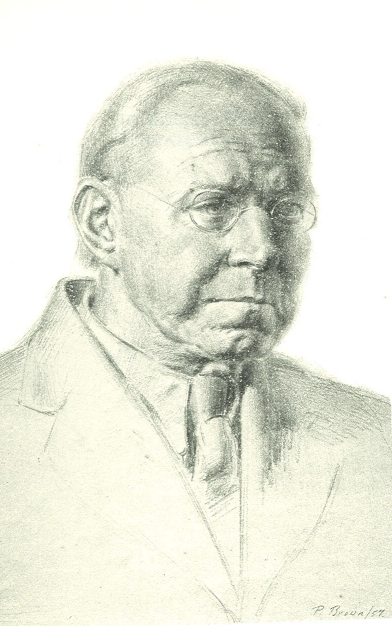
\includegraphics[scale=0.7]{forder.jpg},]
The Forder Lectureship was established in 1985 following a bequest to the 
London Mathematical Society from the late Professor Henry George Forder 
(Professor of Mathematics at the University of Auckland 1934-55). 
Under the terms of this Lectureship, every two years an eminent 
mathematician in the United Kingdom is selected (by the London 
Mathematical Society Council in consultation with the NZ Mathematical 
Society Council) to tour New Zealand for a period of three to four 
weeks and to give lectures in the six NZ university towns.
\end{window}\par

\par\indent
I am in good company. The previous Forder lecturers were:
\begin{itemize}\itemsep0pt
\item[1987:] Christopher Zeeman
\item[1989:] Michael Atiyah
\item[1991:] Peter Whittle
\item[1993:] Roger Penrose
\item[1995:] Elmer Rees
\item[1997:] Ian Stewart
\item[1999:] Michael Berry
\item[2001:] Tom K\"orner
\item[2003:] Caroline Series
\item[2005:] Martin Bridson
\end{itemize}

I didn't find this list anywhere. I Googled ``Forder lecturer'' and found
various references, on individuals' homepages or committee minutes, which
finally allowed me to piece together the complete list. Also the factual
information about the Forder lectureship was in some old NZMS minutes.

According to Stephen Huggett, the money from the original bequest has
run out and the LMS will have to decide whether to use its own resources
to continue the scheme. This doesn't affect my trip, though.

I sent Gaven Martin (the NZMS president) a list of titles and abstracts
of seven talks, which got expanded to nine in March. The titles were:
\begin{enumerate}\itemsep0pt
\item Sudoku, mathematics and statistics
\item The random graph
\item Oligomorphic permutation groups
\item Orbit counting for colourings and flows
\item Asymptotics of incidence matrices and $2$-covers
\item Combinatorics of permutations
\item Isometries of the Urysohn space
\item Cores, hulls, and synchronization
\item Scenes from mathematical life
\end{enumerate}

I am on sabbatical for the calendar year 2008. This should mean that I am
rather less busy than usual, but in fact my time seems to be filled up. 
Apart from this trip, I am spending the first six months at the
\href{http://www.newton.cam.ac.uk}{Isaac Newton Institute} in
Cambridge, directing a programme on \textit{Combinatorics and Statistical
Mechanics}. The Institute staff are amazingly competent, and remove
most of the administrative burden from us, but there is still a certain
amount to do. Also, of course, we are there to make mathematical progress,
and there has been quite a bit of this! At the same time I am a visiting
fellow at \href{http://www.cai.cam.ac.uk}{Gonville \& Caius College};
my only duty there is to give three or four lectures to the mathematics
students at the college. This gave me the opportunity to rehearse some
things that will be in my Forder lectures, especially the last title above.
(The eighth came about as the result of a little mathematical adventure in
January.)

The initial arrangements were a little bit haphazard. I booked
flights to and from Auckland and picked up a few clues as to my movements in
between. By mid-March I had a schedule: Palmerston North (a few days to get over
the jet lag), Otago, Canterbury, Wellington, Palmerston North again, Waikato
and Auckland, a few days in each and a free few days somewhere towards the end.

Rosemary will come with me. She had an operation in January and the
post-operative treatment finished at Easter. The intention was that she would
have a nice restful holiday -- but of course, when the New Zealand
statisticians heard she was coming, many of them wanted her to visit, and
she will be almost as busy as I. (The Forder deal allows either an upgraded
plane ticket or an accompanying person.)

I had to be very careful that the travel agent sent us via Hong Kong and
not LA (after the experience of my last trip to New Zealand, when the
Americans treated the plane rather like a cattle truck). After the initial
booking, Eamonn O'Brien invited me to stay a few extra days in Auckland;
the travel agent nearly managed to send us back via LA at this point!

\begin{window}[1,r,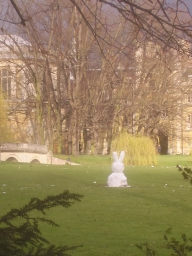
\includegraphics[scale=0.5]{bunny.jpg},]
At Easter, we bought maps and a guidebook and started thinking about the
trip, and I prepared files for the public lectures. It all started to seem
more real. After some appalling weather in mid-March including heavy snow
on Easter day (which led to the appearance of a white Easter bunny on the
Trinity backs), the weather started improving on the last weekend in March,
just before we went. The blackthorn came into blossom in a great hurry, the
sun made sporadic appearances, and it finally felt that spring was on the
way (but not for us -- or at least not yet).
\end{window}

Just before we were to leave, Eamonn asked whether I would be prepared to
add a third talk in Auckland (a public lecture on Sudoku), and could I send
him an abstract, photo, and CV. I collated all the information so far into
a ``schedule'' file, and printed out summary sheets of the two public lectures.

\section{The journey out}

The flight was in the evening of Tuesday 1 April, so neither of us showed
our face at work during the day. (I was a bit tempted; having found how
to compute Galois group in \textsf{GAP}, I calculated that the ``interesting 
factor'' of the chromatic polynomials of $K_{2,n}$ are symmetric
groups for $n\le16$, and had half a mind to circulate this before
leaving.)

We set off for a leisurely trip to the airport, but both trains came
promptly. In the District Line carriage, there were no advertisements,
their place taken by an official-looking notice from Transport for London
explaining that, as part of the ten billion pound upgrade, advertisements
are being removed from tube trains, and hoping that this would improve our
travelling experience. An April Fools joke, we wondered, or possibly a
subtle piece of election campaigning by Boris, persuading us that Ken 
wastes our money on such irrelevancies?

At the check-in desk, some problems with technology: my passport wouldn't
scan, the printer wouldn't work, and then the girl gave us seats five
rows apart by mistake. But finally all was done, we were through security
and passport check, a snack at a rather crowded O'Neill's, and then off
to the departure gate with still more than an hour to spare.

We left promptly. After dinner, I watched about half a movie (``I'm not
there'', from their self-selection system), then settled down to sleep,
and managed a few hours' fitful doze. Then a glance out the window showed
the approaching dawn, with a planet (probably Venus) and the last waning
moon riding just above a band of clouds.
A bit later the whole side of the plane was
bathed in brilliant sunshine. The cabin attendant wanted to keep the
windows shut, like the drapes over a parrot's cage, but by stooping down
I managed to keep my eye to the window and watched an extraordinary
landscape passing below: geometric fields, square, round, or a Young
diagram with a corner cut off by a long straight road; winding rivers
with many oxbows; rugged moutains with lines of snow like some alien
calligraphy; hills like ribs breaking through the plain; ice-covered
round lakes. Mostly the scene was wonderfully clear, but occasionally
it was veiled by light cloud.

The effect of this kind of scenery can't be had from the occasional glance
out the window; it is necessary to sit with your eyes glued to it. Later we
swapped places and Rosemary watched a breathtaking, huge, snow-covered
range of mountains, presumably the northern edge of the Tibetan plateau.
I had no desire to go back to sleep at what was by then the middle of the
day (Hong Kong time), so I watched the rest of the movie and started on
the first part of ``The Lord of the Rings'' (partly as an introduction to
New Zealand scenery). Breakfast and the start of the descent came with
the fellowship in the Mines of Moria, where I had to leave them for a
while!

Hong Kong was much more civilised than Los Angeles: one security check
accomplished quite quickly, then the freedom of the departure lounge.
The airport had a hanging sculpture consisting of multiple icosahedra
made out of metal struts and fluorescent lights, but it was switched off.

Back on the same plane for the second leg, I had dinner (and saw the
Fellowship of the Ring to its end) and then managed
about six hours sleep until I seemed to be definitely awake. Out of the
window, Toowoomba and Southport were both clearly visible (Toowoomba
unmistakeable from the winding road leading up the Range) as we flew
just south of Brisbane. Dawn came over the Tasman Sea at about the same
time as breakfast.

\begin{window}[1,r,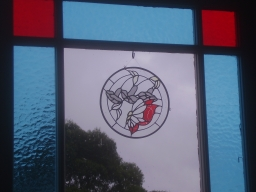
\includegraphics[scale=0.5]{gavenhouse.jpg},]
Off the plane, through immigration (very easy), customs and biosecurity
(slightly more complicated; they insisted on washing the shoes I had
walked by the Dollis Brook in last Sunday). Out of the gate, and nobody
waiting. I wasn't worried; indeed, when I got back from a visit to the
toilet, Gaven was there looking out for me. He drove us to his
extraordinary house, a castle full of wonderful furniture and clocks, on
the top of a hill in Albany on the North Shore. 
One puzzle was resolved, how he could look after us in Auckland while working 
at Massey University.  (The University now has a campus in Albany, and Gaven 
and his wife were made offers they couldn't refuse to move there.)
\end{window}

After a shower, fresh bread and coffee, we felt much more human! Gaven had
to go to his office in the afternoon, so left us the run of the
house.

Gaven had told us that we could walk a kilometre up the road to the main
road, or five or six kilometres in the other direction, or take a steep
muddy path down the valley. We went for the second option and set off
along the road, seeing a magpie-like bird with a shiny blue-green tail. Many
Australian trees here: as well as eucalyptus we saw banksia, bottlebrush
and Norfolk pine.

After walking for about half an hour we came to a crossroads, and thought
about turning back, but we saw a sign saying ``Albany Heights Scenic Reserve'',
and a little path leading off into the bushes. We thought we would do
a quick turn around this and then head back.

Just as we were about to take the path, a car pulled up and the driver
hailed us. It seemed that he was personally responsible for the path,
and encouraged us to take it, telling us that on the way up it was metalled. 
We found out that it was the steep muddy path down the valley, and the 
metalling was incomplete and only started after all the hard work was
over; but it was well worth the effort.

\begin{window}[3,r,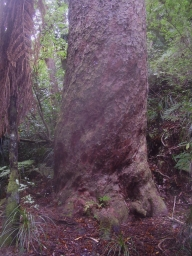
\includegraphics[scale=0.5]{kauri.jpg},]
It descended via steps hewn into the clay (and very slippery after the
recent rain) to a little patch of rainforest, with tree ferns and palms.
Several small chattering birds flitted among the trees, flying acrobatics
and fanning out their triangular tails. A bird hung upside down; not sure
whether the same species or not. A couple more birds were heard but not
seen: one with a characteristic chiming call, but close up we could hear
a fine repertoire of chattering and clicking as well; and another with a
very sweet bell-like song. 
At the creek at the bottom, we found a huge trunk of a kauri tree stretching
up high above our heads. 
On the way up we found many more kauri. We also
found pink flowers on the ground and saw a tree with bright red flowers,
and several kinds of toadstool.
\end{window}

Back along the road, we arrived with our clean clothes quite muddy, and
sat on the front porch letting the mud dry until Gaven came home. He ordered
Thai food and went to pick it up; we tucked in happily. About 7pm Rosemary
suddenly crashed out and we took ourselves off to bed. I slept soundly until
1am, but then my ankle (which had gone again late in the day) was hurting and
I only managed fitful naps and some factorisation of polynomials until morning;
but Rosemary slept soundly all night.

The next morning we met Dianne over a leisurely breakfast, just back from a
conference in Coff's Harbour and a visit to her father in Mackay. We went
out with her to pick figs, and then she picked up a couple of pockets full
of feijoa, which we sampled -- a rather easily acquired taste, I think, though
Gaven professed not to like them. From the verandah we watched a kingfisher
on a wire. After as much displacement activity as
she could reasonably manage, Dianne went off to her lab (she has twenty
postgraduates and quite a few postdocs in her ecology/conservation lab at
Massey), Gaven to his office, and we were left to have an easy morning.

The ``white toy'' (my Asus eee-pc) proved its worth once again. It easily
connected to the wireless network in the house, without even needing to
ask a question, and then both Firefox and ssh worked flawlessly. The Windows
laptop, on the other hand, complained about this, that, and the other, and
after a lot of effort I was finally defeated because it couldn't proceed
without knowing the ISP. So we were able to read our email (with a bit more
information about the rest of our trip), make train bookings (we will take
the train to Greymouth and back, then train to Picton and ferry to Wellington,
and then to Hamilton in three stages) and a guesthouse for one night in 
Ohakune on the way. So everything is sorted as far as  Hamilton now.

\begin{window}[1,r,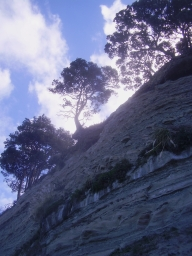
\includegraphics[scale=0.5]{longbay.jpg},]
When Gaven came back he whisked us off to the beach, at Long Bay. I knew,
looking at the beach and the water, that the sea would be good for my
ankle, and so it turned out. I rolled up my trousers (having not had the
wit to change into shorts before we went), hobbled down to the sea, and
let the warm Pacific wash around my foot and shin.
The beach itself was backed by low grassland, but there were high mudstone
cliffs at each end, with the native pohutukawa trees precariously perched 
on top or lying, still growing, at the foot (in contrast to the imported 
pines, which had splintered and died as a result of a cliff fall). 
\end{window}

There were many shells of varied and subtle
colours, and Rosemary found a bluebottle on the waterline. We saw various
gulls, including black-backed and black-billed (some juvenile) and several
pied oystercatchers.

Then home where Dianne cooked rack of lamb and baked the figs we had
picked that morning, and also spent some time sitting with the rest of us
on the verandah. We discovered that the mostly black bird with turquoise
sheen we saw yesterday, and the amazing singer we'd heard, are one and
the same: they are tui, of whom several came and sat in the tree and gave
us a concert. As well, there were blackbirds, chaffinches, and sparrows,
all introduced. We also learned that, unsurprisingly, the birds that
fanned out their tails are fantails.

I also learned a couple of things about the Forder lectureship from Gaven.
Forder died sometime between 1970 (when a book in his honour was produced)
and 1977 (when Gaven was a student at Auckland). Also, his perception,
shared by others here, is that, rather than the Forder money running out,
it was put in the LMS general account and no track was kept of it.

We ate formally in the amazing dining room, with 
candles lit. After dinner, Dianne's mother and stepfather came around
and we talked for a while, until Rosemary and I made our excuses, having 
an early flight to catch.

Gaven's hospitality has given us the ideal way to get over the jet lag,
and has set me up so well for what follows -- thanks Gaven and Dianne!

\section{Dunedin}

The next morning, Gaven was up when we came downstairs, and made us coffee
with his wonderful espresso machine. The taxi arrived on time; it seems
that this is his regular taxi, which had brought Dianne from the airport
two days previously. With little traffic, we made good time.

The driver had a card on his windscreen saying ``Falun dafa is great: Truth,
Compassion, Tolerance''. So I was not surprised when, after turning off the
motorway, he started talking to us about Tibet and the Olympic Games,
He told us that on his last visit to China to see his mother he had
been imprisoned for a month and tortured, and finally deported back to 
New Zealand. We found ourselves very much in agreement, but he surprised
me by predicting that the Communist Party in China will collapse during
the Olympics.

Our plane had been borrowed from another airline (Thomson I think) who
had borrowed it from yet another; the exit signs were in Spanish and
the plane was unused to flying to cold places according to the steward.
We had window seats to Dunedin, but there was nothing but cloud to be seen
most of the way, except for one brief moment when the Captain drew our
attention to the fact that Mount Cook was visible -- in the distance, and
on the other side of the plane, so just a glimpse through the opposite
window -- until we came down through the clouds over the coast just north
of Dunedin, and turned inland with a good view of the city and harbour,
up to the airport.

\begin{window}[0,r,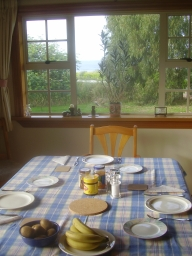
\includegraphics[scale=0.5]{brunch.jpg},]
After landing, passengers were told that they could turn on their cellphones.
But this order was later countermanded: another plane was using the airbridge,
and we had to walk across the tarmac, where phones are not allowed.
As we came in, there were Tank and Karen waiting for us.
They whisked us off to their house, where Karen gave us a tour of the
garden while Tank made brunch. Every plant in the garden has a story,
and many had been given by or were associated with friends. She had just
retired, and is looking forward to putting in more time in the garden;
she apologised for the sparseness of what seemed to us a blaze of colour
and growth, with the melodious birdsong from the trees around, including
a familiar sound: an (Australian) magpie. Then we made a leisurely and
delicious brunch of kedgeree, cheese muffins, scones
and jam (all freshly made), coffee and juice.
\end{window}

After brunch, we went for a walk on the
beach. Quite a contrast to yesterday: silver sand, few shells, sea deep
blue, piles of large kelp. There were black oystercatchers and stilts.
(The bird book says that NZ oystercatchers are black but the northern
ones have a pied phase.) The day was turning clear and warm and the
beach was ours alone for most of the walk.

\begin{window}[1,r,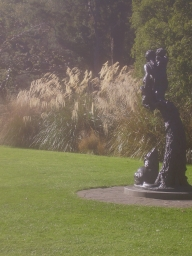
\includegraphics[scale=0.5]{dunedinbg.jpg},]
Then into town, where Karen had a lunch party with her former colleagues.
Tank took us to the motel. After a break while he went to his office and
we did some laundry, we walked in the 
\href{http://www.cityofdunedin.com/city/?page=sites_bg}{Botanic Gardens},
up the hill and
through the South African section, rhododendrons, and native bush. Glorious,
with the day just perfect: sun warm, sky clear, air with a hint of chill,
and different but even more melodious birdsong.
Back to the motel, past a solitary Moeraki boulder set in concrete.
Tank picked Karen up, we walked towards town and
had huge bowls of delicious and sustaining noodle soup at the Apsara
Cambodian restaurant.
\end{window}

Next morning, the clocks went back, so we had a leisurely morning. We had
coffee and showers (Tank had kindly bought us some real coffee, and the
motel room had a tiny coffee pot), then I revised my first talk and
copied photos onto the laptop.

We walked in to town for breakfast.
The Governors should have been open but had a ``Closed'' sign up. Someone
bolder than we went in and asked -- the staff hadn't shown up. So we went
to Capers instead and had a fine breakfast of pancakes, smoothies and coffee.
Then we walked to the Octagon (where we bought postcards at the tourist
information) and the railway station (where Rosemary booked on the Tuesday
morning Taieri Gorge trip). The tourist information office was virtually empty
when we walked in, but just after us came a huge party of tourists who tried
to pay for their purchases with U.S. dollars. At the station, the volunteers
who run the railway were in a state of shock, having had to put extra
carriages on the train to cope with an unexpected large party.

Walked home, with a stop at a shop selling cheap
trousers and very cheap binoculars. I went out for sandwiches.
After lunch, Derek and Marilyn Holton picked us up for a birdwatching trip
to the peninsula. And what an afternoon we had -- even Derek as an old hand
was impressed.

On the way out, and often throughout the day, we saw harriers, near or far.
First we went to Hooper's Inlet and drove right around it. We saw white-faced
heron standing or flying, oystercatchers, stilts, paradise ducks on sea or
land (the males with black heads, the females white), mallards, teal, a
little shag on a post in the water, half a dozen pukeko (swamphens) by a
small stream on the other side of the road, and a couple of black swans.

\begin{window}[1,r,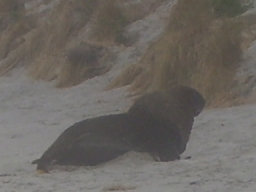
\includegraphics[scale=0.5]{sealion.jpg},]
Then we drove to Allan's beach, between the inlet and the ocean, hoping to
see penguins moulting, but the tide was too high to get around the point.
There were a couple of black-billed gulls on the almost empty beach. But
there, taking his ease halfway along the beach just above the highwater mark,
was a huge sealion. We went over to look, not going too close, but he was
not much interested in the phoho-opportunity and mostly just lay there looking
like a big piece of driftwood.
\end{window}

From there we went over to the harbour side of the peninsula, where we
could see a huge cruise ship at anchor. Derek said that if the weather
is too bad for the cruise ships to enter Milford Sound, they come round
and moor at Port Chalmers instead. This explains the vast number of people
in town this morning and the chaos they had created.

\begin{window}[0,r,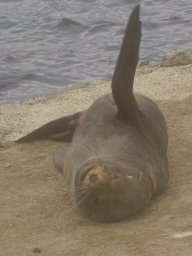
\includegraphics[scale=0.5]{seal.jpg},]
We drove to Pilot Beach. There were a couple of blue penguins moulting, but as
they hide away in their holes to do it there was not much to see, just a 
blue-grey blur in the darkness. But two big seals were lying on the ground
by the path, and while too lazy to move, would raise a flipper from time to
time. Then a large dark-coloured bird, almost certainly a giant petrel, 
came swimming
by. There was a big crowd of black-billed gulls, who got extremely perturbed
by this, and a patrol went out to see it off, which they did rather viciously.
\end{window}

There was time for a cup of tea before the Penguin Place tour Derek had
booked us on, so we went up the hill to the albatross colony. The woman
running the tea shop greeted us with ``I've been cleaned out!'' A party from
the cruise ship had descended on her. But she had a few cakes left. No sign of
any albatross flying, but we went in for tea and cake and sat by the window.
Right on cue, a solitary albatross came soaring over the hill and circled
while we finished our tea.

I read in a book we acquired later in the journey an astonishing and
inspiring fact about the albatross. The young do no flying practice; they
simply step off a cliff into the wind, and then don't touch land again for
three to six years.

\begin{window}[6,r,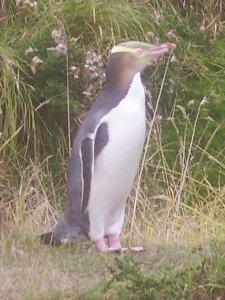
\includegraphics[scale=0.5]{penguin.jpg},]
On to \href{http://www.penguinplace.co.nz}{Penguin Place},
where we were given a quick sumary of the yellow-eyed
penguins' life cycle before getting on the bus to head for the penguins
themselves. The weather was threatening rain but held off for our tour.
The penguins are monogamous with a relatively low divorce rate, and they
are tagged and given names so we can hear their life stories.
Most of the
penguins we saw, having hatched their chicks, were either moulting or just
finished moulting, so either extremely scruffy or extremely neat. We saw
many penguins, including some that the guide didn't recognise; for one of
these, he read the tag number and radioed it to base, and was told that it
had been tagged as a chick two years ago and this is the first sighting 
since. This was just after we'd seen one penguin call its mate out of
the shelter, when they put on a long display of the neck-stretching that
means ``How pleased I am to see you!'' and then headed, waddling and bouncing,
up the steep hillside until they disappeared from view behind the bushes.
\end{window}

We watched penguins coming out of the sea after a day's fishing. Mostly they
stand on the beach for some time to get their breath back; but one pair,
whom we'd seen ``porpoising'' in the waves (this means just what it sounds
like), came out of the water and sprinted up the beach into the dunes.
The guide said that they had probably seen a shark or sea lion and were
terrified.

There were a couple of seals stretched out on comfortable beds of seaweed on
the beach, and several more lying on the grass (or rather, where the grass
had been before their body oil killed it off).

Back to base, and into the car to drive back to town, and the rain finally
started seriously, having so kindly held off all afternoon.

Derek and Marilyn took us to an Italian restaurant called Etrusco in what
had been an elegant Edinburgh-style first-floor tea-room (for Morningside
ladies, as Rosemary put it). The service wasn't very good (they managed to
ignore us for long periods), but the food and wine (a New Zealand Malbec)
were well up to scratch.

The next morning, breakfast in Capers again, and sharp on the dot of 9 there
was Peter Johnstone to pick Rosemary up for the day. I went in to the
University, and found Karen in Tank's office, just about to leave. We had
a lot of discussion about the sad state of universities, and also during
Tank's absence managed to revise my talk a bit, read my email, and had lunch
in the small caf\'e downstairs in the same building.

After a few alarums and excursions (e.g. Tank had to attend an emergency
meeting on a student caught cheating in a test), it was time for my talk
on \href{sudoku.pdf}{Sudoku, mathematics and statistics}. I couldn't 
run overtime since there was a lecture in the same room immediately 
afterwards, and perhaps I erred a little on the side of brevity; but it 
was well received. There were 14 people present.

In the afternoon I went back to the schedule, which is now clear as far
as Wellington. I was dismayed to find that for Palmerston North I didn't
even have the name of the contact person, let alone details of 
accommodation and talks. For Hamilton I have all but the last of these.
With Tank's help and that of Charles Little I got the name and email of
Matt Perlmutter in Palmerston North and sent him an apologetic email.
Ernie Kalnins has promised that the secretary will send me the talks
for Hamilton soon.

In the evening Tank and Karen took Rosemary and me to dinner at the
Indian Summer restaurant. It was really good: portions just the right
size and beautifully cooked, mango lassi to die for. But we were too
full for dessert. (Had they had kulfi I might have been tempted.)

The next morning, after another really good breakfast at Capers, I went
with Rosemary to the station and put her on the 
\href{http://www.taieri.co.nz}{Taieri Gorge Railway}, then returned
to the motel, picked up my stuff, and went in to the department. There was
a reply from Matt, so Palmerston North is now sorted. Tank told me about
the permutation avoidance problem that several people here are working on.

I had lunch of sushi with Tank, then gave my second talk on
\href{scenes2.pdf}{Scenes from mathematical life}, to 20 people.
It went well except for a technical glitch in the middle when the screen
went blank, but we soon got that fixed.

After that I read my email and found a response from a new contact person
in Hamilton (Kevin Broughan), so that part of the schedule is now sorted.
Also, I booked a motel in Paihia on the Bay of Islands for the four days
between Hamilton and Auckland. The only technical thing to be done now is 
to book buses Hamilton - Paihia and Paihia - Auckland.

After Tank had showed me his and Karen's stunning photos of Easter Island
and Chile, I walked beck to the motel. Derek and Marilyn picked us up at
7:00 for dinner in the Bacchus Wine Bar. We ate very well indeed: I had
blue cod, then lemon cheesecake, and we had a pleasantly fruity Carrick
sauvignon blanc from central Otago, and talked about many things including
Julian Jaynes' \textit{The Origin of Consciousness in the Breakdown of the 
Bicameral Mind}. Too tired to pack when we got back, so we did the crossword
and went to bed.

\section{Christchurch}

The morning dawned clear and beautiful, with just a few tiny white clouds.
A last breakfast at Capers, and the job of packing (things no longer fit,
and a new suitcase will almost certainly be necessary). Then Tank came and
picked us up and took us to the University where we had the use of a computer
and a morning to read email once more. He went off to give a lecture, and
Karen came to take us to the bus station. Check-in was remarkably informal:
two plastic boarding passes with no journey-specific information on them,
and no announcements. Tank and Karen have looked after us so well in
Dunedin!

The most mountainous part of the journey was right at the start, with a
pull up the very steep hill overlooking the valley of the Water of Leith,
with houses perched precipitously on the cliff above the old quarry on the 
other side; then down to the inlet at Waitati, where there were a few
waders on the mud but too far away for identification; then up another
steep hill on the other side.

\begin{window}[2,r,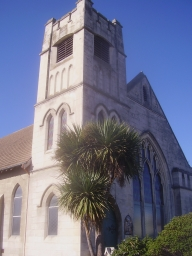
\includegraphics[scale=0.5]{oamaru.jpg},]
The first leg, to Oamaru, was through pretty, undulating country with sculpted
hills and tiny settlements. We saw quite a few harriers. The farms had mostly
sheep, but some cattle, goats, deer, and alpaca. The trees were colouring for
autumn, most noticeably the lines of poplars. One nice stretch took us along
Katiki Beach, just before the famous Moeraki Boulders; we saw a sign to the
boulders, but didn't get near enough to say beyond a doubt that we saw them.
We made a refreshment stop
in Oamaru, where the bus company shared premises with a nice old-fashioned
caf\'e where I had a very good (but solid!) mutton pie. We had time to 
walk down to the sea, past one of several churches made of the characteristic
Oamaru limestone. On the shore, there was an old station with some strange 
piece of machinery (including one passenger carriage) on the track. 
(Later we saw one party of track workers laying ballast, and later still a 
freight train with quite a big load.)
\end{window}

Soon after Oamaru we crossed the Waitaki River. This was one of several
very wide braided rivers we saw which were carrying almost no water but
looked as if they would be raging torrents in the time of snow-melt.

The crossing took us out of Otago and into Canterbury, and the start of the
Canterbury Plain. Almost immediately the sky darkened: we were under a pall
of smoke from burning stubble, held down by a temperature inversion, so that
only the nearest mountains were dimly visible through the haze, and out to
sea was a filthy brown smudge. At Winchester, the smoke was so thick that
the sun went red. So much for New Zealand's green credentials! This was
the Shire in the hands of Mordor. We also saw the very high density that
sheep and especially cows are kept at here, and were told later that the
huge irrigators suck the aquifers dry and run-off from the intensive farms
pollutes them with nitrates.

The plain, especially after Timaru, was much more densely populated, with
reasonably substantial towns quite close together. Thick pine hedges
presumably acted as windbreaks, but also blocked the view.

As we approached Christchurch, the sun set. The mountains became clearer,
their milky blue standing out against the rich orange of the sky. Crossing
the Rakaia River, we could see one large peak on its own, which may have
been Mt Hutt. A tiny new moon hung in the orange sky. The other side,
over the Banks Peninsula, the earth cast its shadow on the smoky sky.
The towns, and the suburbs of Christchurch, sprawled along
the highway, with huge out-of-town shops and used car dealers.

At the bus station, there was Ben Martin, who took us to the motel, and also
told us that a party including Angus Macintyre and Douglas Bridges, were going
out to eat and we were invited to join them. We phoned Angus and set this up,
and then Ben kindly gave us a lift back into town to the restaurant.

We ate at Restaurant Indochine, which did Thai-influenced gourmet food.
After shared starters (with especially good spare ribs), I had pork belly.
We got through quite a bit of wine, especially at our end of the table.
A lot of reminiscences -- Douglas had been a student of Robin Gandy and
Michael Dummett in the early 1970s, and did a good imitation of the inimitable
Robin.

\begin{window}[1,r,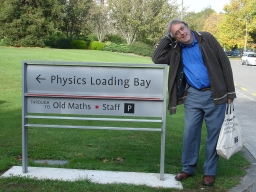
\includegraphics[scale=0.5]{oldmaths.jpg},]
The next morning, after a breakfast much like our usual at home but seeming
very modest in comparison to recent days, we walked in to the Mathematics
department. On the way in, I had my picture taken leaning on a sign saying
``Old Maths - Staff''. In the department we found Ben, who took us to our 
respective shared offices.
There were computer problems: the firewalls are so secure that you can't
even access Google from the desktop computer without having the IT person
come and spend a long time typing in complicated instructions. 
But at last it seemed to work -- though later on, trying to upload a 
reference to the AMS jobs website turned out to be a nightmare; 
in the end I am not sure if both pages were uploaded
and had no way to find out without emailing the AMS webmaster.)
\end{window}

On what turns out to be the anniversary of the Wahine disaster,
I got an email saying that there are problems with the ferries, and we will
be an hour later in Wellington. Everything else fine. Kevin will book a bus
from Hamilton to Paihia at a civilised time of day.

We had lunch in the Staff Club, a fine old building formerly the house
of the Rector, and then walked randomly in its extensive and peaceful
gardens, where a couple of late rhododendrons were still in flower.

In the afternoon Ben and I talked about random 2-in digraphs, then it was
time for my talk. We couldn't get the built-in computer to respond, so it
was the white toy to the rescue again! 20 people came, many of them students,
and it went well, with interesting questions afterwards. Then a cup of tea 
and some further talk, and so back to the motel. 

We ate in the motel dining room -- there is not much else within walking
distance. 

\begin{window}[7,r,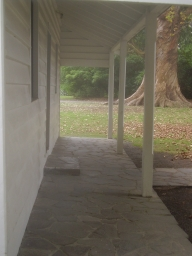
\includegraphics[scale=0.5]{riccarton.jpg},]
The next day was the low point of the trip so far. In the morning, 
I felt quite ill (not from dinner, I think), so
had to scale down my proposed sightseeing somewhat. I went to the Riccarton
Bush and wandered around the little patch of original New Zealand bush. The
most striking thing was the birdsong, an intense mixture of melody, warbling,
and other sounds quite unlike what I have heard elsewhere. But I couldn't
stop for too long, as I felt like throwing up, and thought that this wouldn't
really be appreciated in a conservation area.
The rest of the walk was rather dire -- I went to the station (and saw two big
freights go past, one in each direction), and to Hagley Park (but no time for
the Botanic Gardens), and then back to the University by a somewhat indirect
route, trying to keep off the big roads of which I had had more than enough.
I got a sandwich and managed to eat it in the Maths common room without
throwing up, then went to my office, where I couldn't manage to log on to my
account (presumably the fix provided yesterday by the IT person was only
short-term). I tried to have a short nap, but was interrupted by Douglas
Bridges coming for the money for dinner the first night.
\end{window}

I gave my talk on the random graph to 13 people. Though I felt rather
spaced-out (Ben had got me a couple of Panadin from the secretaries, which
I had taken before the talk), I think I was coherent, and there were some 
good questions afterwards. We had tea in the common room, and then went over
to the Staff Club where everyone drinks beer on Friday night. I had a cold
imitation-bitter, which I drank very slowly, waiting for Rosemary and her
host Dave Saville who were due to take me to dinner at 5:15.

When they hadn't shown up by 6, I went back to the motel. Perhaps there had
been a change of plan, I thought, and they emailed me about it, and of 
course I didn't get the email. I even tried to subscribe to the service
providing wireless internet in the motel; but you need both a mobile number
and a New Zealand landline or it won't accept your application.

They showed up at 6:15, having fallen behind schedule. We drove out to
Dave's place in the country where he has a bit of land, runs a few sheep,
and grows vegetables, with his wife Sandra and daughter Jessica, a very
self-possessed teenager who works for market research. The plan had been
to have a guided tour of the property first, but given that dinner was ready
we decided to eat. It was a delicious dinner of roast lamb with homegrown
vegetables followed by a large assortment of desserts. I didn't disgrace
myself until after the meal when finally what had been waiting to happen
all day caught up with me: I rushed to the bathroom, just making it in
time, and was quite violently sick.

Afterwards, having said I'd come on the tour, it was just assumed that I
would come. First we took some hay to the first paddock of sheep to
attract them over so we could see the ram; but he was shy, and let the
ewes come up first, while he skulked at the back. We looked at the other
paddocks, the vegetables, fruit and flowers, then sat by the fire and talked
for a while, then he drove us back to the motel. Jessica gave Rosemary a
small bag of her own cherry tomatoes, and came with us for the ride. I 
perked up enough to call a taxi for the morning, on the number that Jessica
had spotted for us on a taxi in front of us on the road.

Up early the next morning to have breakfast before the taxi came, but 
breakfast was late and the taxi early and we were still eating when it came;
but we got away in time. A quick journey to the station, and soon we were on
\href{http://www.tranzscenic.co.nz/services/tranzalpine.aspx}{our way to 
Greymouth}.

Out over the rather dull Canterbury plains with the view blocked by hedges
and the grey clouds low in the sky.
A thought struck me. It is usually assumed that Lewis Carroll's vision of
Wonderland as a country divided up by hedges and ditches was based on
the view of Otmoor from Beckley, which actually doesn't look much like
that. But he was a fellow of Christ Church, where the association for
settling Christchurch and the Canterbury plains had been set up not long
before; perhaps it was talk of this in the common room that had inspired him?

We made various stops to pick up or set down passengers, but at Springfield
they had a longer stop to put on an extra locomotive, and we were allowed
out for five minutes. The buffet sold ``The pie you can trust''. Somehow, the
issue of trusting a pie never occurred to me before!

After Springfield we began climbing. The clouds cleared to give blue sky and
sun, with just a few white clouds drifting as mist about the tops of the huge
mountains. We soon came to the first of a series
of spectacular views of the Waimakariri River, in brief gaps between
tunnels. The river flowed strongly in a small channel of its wide stony
bed below rugged mountains.

\begin{center}
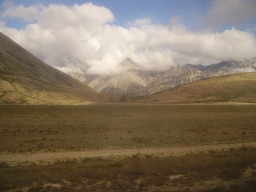
\includegraphics[scale=0.5]{clouds.jpg}\qquad
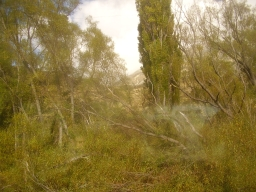
\includegraphics[scale=0.5]{alpine.jpg}
\end{center}

\begin{window}[1,r,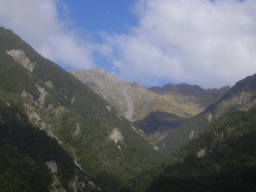
\includegraphics[scale=0.5]{arthurs.jpg},]
We turned off up Broken River, which we crossed
on an impressive viaduct, and then up a smaller creek. There were many willows,
with leaves much yellower than those we'd seen before, and a poplar which
reminded me of the tree in \textit{The Mabinogion}: the trunk had split, and
one side was entirely green while the other was bright yellow.
At Craigieburn we had
a short stop to cross a coal train. Rising to Arthur's Pass, and crossing
the Waimakariri (which had risen to our level), the vegetation changed
to conifers. Another five-minute stop, whose real purpose was made clear by
the ugly heaps of cigarette butts under the shrubs in the gardens on the
platform.
\end{window}

Soon after, we went through the 8.5km Otira tunnel and out onto the western
side of the Alps. The vegetation was different again, much more lush in this
high-rainfall area. Coming into Moana, there was a good view back to the
mountains behind Lake Brunner. After this we were in what I'd imagined as
much more typical New Zealand scenery: very green, scattered cattle and
farmhouses. But soon we went through a valley that was almost sub-tropical
in appearance, with swampy regions of ferns and flax plants. These two
types of scenery alternated the rest of the way to the Grey River and down
to Greymouth.

\begin{window}[0,r,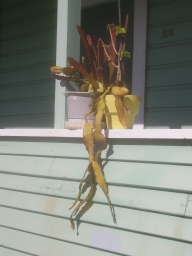
\includegraphics[scale=0.5]{greymouth.jpg},]
The town of Greymouth belied its name: not at all grey, 
and not at all workaday as the
guidebook claimed, it lay sleepy and quiet in warm sunshine under a 
cloudless sky, with colourful painted wood buildings and fine views of
distant mountains. We walked along the floodwall to the very un-busy harbour,
where three cormorants sat on three posts next to the slipway, then back
past the colourful Duke's Backpackers building. No time for museums, shops
or pubs (unfortunately!) as we had just an hour before the train left.
\end{window}

On the way back, with the window seat and facing the other way, I got quite
different impressions. I attempted a few photos from the moving train. For
this, the usual rules have to be forgotten; no foreground! One should look
ahead to check that no trees are coming up, but the digital camera has a
small delay, so sometimes the best-laid plans are foiled. But some pictures
turned out tolerably well.

\begin{window}[1,r,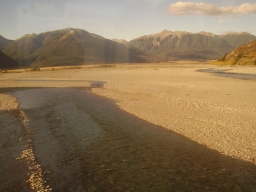
\includegraphics[scale=0.5]{waimakariri.jpg},]
The train took a winding course up a valley, seeming to head for impenetrable
walls of mountains but going round a corner at the last minute, and at one
stage was heading more-or-less west. But we came at last to the Otira Tunnel,
lading to Arthur's Pass where we had a short stop. Then back past the 
amazing views of the river, not so sharp now with no sun on the bottom
of the valley, and across the plains back to Canterbury.
\end{window}

Birds seen: magpies, harriers, pukeko, plovers, paradise ducks. Also cows
with markings like Wessex Saddleback pigs, and huge numbers of beehives --
sometimes it was clear that the bees were foraging in huge stands of gorse
still in flower.

We walked back from the station, stopping for dinner at a Lebanese restaurant
(really just a kebab house) on Riccarton Street, and had an early night.

\section{Wellington}

The alarm woke me after a good night's sleep. For the first time this trip,
I awoke without any aches, pains or grumbles. The taxi arrived early again,
and soon we were off to the station, with the Morning Star shining over the
city street lights in a beautifully clear sky. At the station we were in
good time for
\href{http://www.tranzscenic.co.nz/services/tranzcoastal.aspx}{the train
to Picton}.

Before we were out of the suburbs, we were into a thick mist, through which
the rising sun loomed mysteriously. After a while it thinned to a low ground
mist, with silhouettes of animals and trees against the silky white. For some
time we were in mist of varying thickness, with no distant views. Sheep near
the railway line scattered in panic at our approach, though this must be an
everyday occurrence for them. We also saw magpies, plovers, and paradise
ducks.

The mist cleared briefly to give us good views of the Hurunui River. Then
through another patch, until we came to the Conway River, where it finally
cleared away to reveal a beautiful sunny day. 

Descriptions of Paradise, Fairyland, etc., all stress the
clarity of the light and the brilliance of the colours; this is exactly how
it was as we went down the Conway Valley. The rich gold of the willow and
poplar leaves, the green coutours of the hills on the other side, tiny
birds clearly visible in the air between.

\begin{window}[0,r,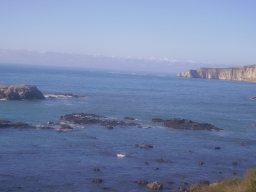
\includegraphics[scale=0.5]{coastal.jpg},]
Then we came to the sea, and decided to go to the open viewing carriage
for a while. We passed deserted beaches, rocky outcrops, headlands, and the
waves breaking on rocky islands. Once we saw dolphins leaping in the waves,
and once I thought I saw a whale leap far out to sea: just a dark smudge
followed by a white smudge, not at all certain. There were seals on the
rocks, a small group of herons on a beach, and cormorants a-plenty.
\end{window}

\begin{window}[1,r,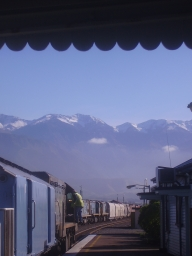
\includegraphics[scale=0.5]{kaikora.jpg},]
After Kaikora, where we made a short stop, we briefly had tall snow-capped
mountains on one side of us and turquoise sea on the other, until we were back
on a rocky coast of headlands and beaches bounded by hills. I saw numerous
seals on the rocks and half-a-dozen herons on the beach. The road was
between the railway and the sea, and we past several roadside crayfish stalls.
Through sand dunes, we turned inland into a region of hills looking like
overgrown green sandhills. The clarity of the sunlight was slightly diminished
by a belt of high wind-tossed cirrus cloud. Past Lake Grassmere saltworks with
its huge piles of salt, and the North Island in view in the distance. Coming
into Seddon there were lots of vineyards, many of them new plantings.
\end{window}

Over sandy hills and past Big Lagoon to Blenheim, with industrial-scale
winemaking, vineyards stretching as far as the eye can see and tended by
tractor. Then up a steep grade over hills covered with forestry plantations,
and down into a long narrow valley with grazing cows and not a vine to be seen,
which we followed all the way to Picton.

We disembarked from the train and went to the ferry terminal to check in.
There had been some confusion over baggage: we were given purple baggage
tags, but the train crew announced that green tags would be transferred
automatically but people with blue tags should collect their bags and
carry them to the terminal. It turned out that we were OK on this.
There had also been some confusion over time: the ferry company had emailed me
that the ferry was an hour later, but when we checked in at Christchurch the
train company knew nothing of this; but on arrival at Picton, they announced
that we had all been notified of the change. 

\begin{window}[1,r,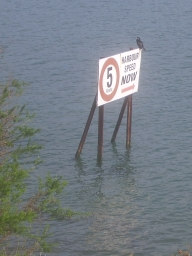
\includegraphics[scale=0.5]{bobsbay.jpg},]
It was indeed an hour later,
which gave us time to walk around the Victorian seaside resort of Picton
and do a short stretch on the Bob's Bay trail. After a while, Rosemary (whose
knee was giving her trouble) decided to wait for a while while I went on.
It was so nice to be able to jog along the track without any discomfort!
Fine views of the Queen Charlotte Sound and back to Picton, and a bit of
bush, where a weka (rather dark-coloured) scuttled off the path into a bush
as I approached but let me come quite close. On the way back, something
stung me on the hand (not too serious -- New Zealand stings are rather mild!)
\end{window}

Back to the terminal, and we had time for a slightly rushed but very nice
lunch before we were called to board
\href{http://www.interislander.co.nz}{the Interislander ferry}.

\begin{window}[1,r,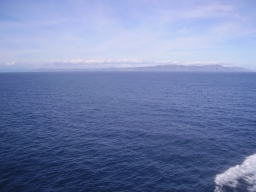
\includegraphics[scale=0.5]{aotearoa.jpg},]
It headed out into a sea as calm as a millpond, with nothing but the
high cirrus cloud in the sky, and a gentle breeze, on the fortieth anniversary
of \href{http://www.wcl.govt.nz/wellington/wahine.html}{the \emph{Wahine}
disaster}. Stunning views down the extraordinary sound, with tiny bays
under wooded hills containing a single house or a small settlement with a
few boats, then more rugged as we got nearer the sea, until we passed some
rocks off the last cape and were into open sea. In front of us was the
North Island, high cliffs with blue mountains behind, stretching and fading
on either side, and above all 
\href{http://en.wikipedia.org/wiki/Aotearoa}{a long white cloud}.
\end{window}

We came gently across the strait and along the coast, entered Wellington
harbour giving a wide berth to the rocky reefs sticking out from every
headland. As we came into the harbour there was a very bright sun dog in
the cirrus clouds. We docked right on time at the Interislander terminal,
and Geoff Whittle was waiting for us.

He took us to our hotel, a serviced apartment in a tall building on the Terrace,
and came back an hour later to take us to dinner at his house (which is
approached down a long sequence of public stairs, which take the place of
roads at many places in Wellington, and along the unlit and overgrown
garden path, so that it became a real adventure). Mike Newman
and Noam Greenberg and their partners were also there. Geoff and Lisa have
a Burmese cat called George who demands loudly to be the centre of attention;
George planted himself on my lap, both before and after dinner, and made an
absolute fool of himself by getting into ridiculous postures while I stroked
his head and neck.

The delicious dinner of beautifully spiced lamb, Maori potatoes (which were
introduced by very early Europeans and taken up by the Maori while they
became extinct in Europe -- one in particular had deep purple flesh and was
absolutely delicious), vegetables, and green beans, and lot of good wine, was
accompanied by hilarious conversation which had us all in stitches. A most
enjoyable evening which saw us fairly late to bed.

In the morning we went out for breakfast. The hotel desk suggested going
through the James Cook hotel to an arcade with caf\'es on Lambton Quay. 
We got
a bit of a shock when we walked down an alley beside the hotel and found a 
sheer drop to the street far below! But in the hotel were lifts down to the 
bottom. We got a good breakfast with a newspaper, only slightly more expensive
than Capers in Dunedin. We were told later that this slope is an 
earthquake-induced slip, and the big buildings on the east side of the
Terrace have their foundations at the bottom of the hill.

\begin{window}[1,r,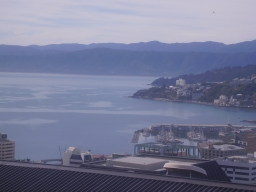
\includegraphics[scale=0.5]{wellington.jpg},]
Then up to the university: along the Terrace past some fine old
wooden houses with beautiful window class, then up the hill past an old
cemetery. We found the Mathematics
Department easily and were shown the way down the convoluted corridors to
Geoff's office, with its amazing view over Wellington harbour. Two labels
on broom cupboards caught my eye: ``Fossilised programmers'' and ``COBOL
museum''.
Geoff had arranged a room (next door to his, with the same view) and a
computer account; everything worked flawlessly right from the start. By the time
I'd made a first pass through three days' worth of email, and found that 
Kevin had sent bus times from Paihia to Auckland, it was coffee time, and
we went over with Geoff and Mike. Later Noam and a postdoc joined us,
coffee became lunch, and we sat there until not long before my talk.
\end{window}

Fifteen people came to the talk and were a really enthusiastic audience.
After 50 minutes I was still in full flow, and Noam (the seminar organiser)
proposed that anyone who needed to could go but the rest could continue
a bit longer. Nobody went. There were several very good questions afterwards.
Then a bit of time to read mail again and catch up on my diary before dinner.

By now it was raining, not hard but persistently. Dinner was in the Yangtse
restaurant, which specialises in duck: the crispy parts wrapped in pancakes,
the flesh stir-fried with noodles and wrapped in lettuce leaves, and the
bones boiled into soup. Nine people dined, and we had an excellent meal.

At one point, talk came round to the Forder lectureship. The view was that
Forder had left his money to the LMS without specifying the lectureship,
which would explain why it was put into general funds and why there was a
delay in setting up the lectureship. It was said that Ioan James had
visited New Zealand for the negotiations -- he was long-term LMS treasurer
so this fits.

Then along Willis Street and Lambton Quay, and back in the lift to the
Terrace. The other town I know which has a lift (and many escalators)
to get you from one part of town to another is Potenza, in south Italy.

Back to Lambton Quay next morning for breakfast, and then off up the hill
to the University, where my second talk was at 11, on ``Oligomorphic Permutation
Groups''. Again it went down extremely well. Afterwards I commented to Geoff
that he hadn't asked for the one talk with matroids in it; he said that the
department is strong on logic and algebra, and that he is happy to hear
about these things! The weather was quite dismal by this time, so Rosemary
came to my talk and then came to lunch in the Staff Club before going off
sightseeing (by which time it had improved a bit).

Back to my office with Mike and Geoff. I had a long talk to Mike about
cores and related things, which of course are right up his street. We tried
to prove some of my conjectures about the complexity of hulls, without
success, and I encouraged him to see whether he has up his sleeve any examples
of permutation groups which are synchronizing but not separating.

Then it was time for coffee. Both the usual place and the Staff Club were
shut, so we went out for a little walk to a delightful coffee shop in a
suburban street opposite an old church, and with views across a valley to
houses clinging to the hill on the other side. We stayed there for a long
chat. Among other things I learned that the floor is made of recycled native
New Zealand timber, for which there is quite a market now that the native
trees are protected.

\begin{window}[0,r,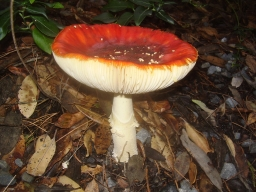
\includegraphics[scale=0.5]{toadstool.jpg},]
Finally it was time to return my key and say goodbye. I decided to go down
in the cable car, so I walked to the cable car station on the edge of the
\href{http://www.wellington.govt.nz/services/gardens/botanicgardens/botanicgardens.html}{Botanic Gardens}. 
It was still light, so I went for a little walk in the
Gardens, to luxuriate in the native birdsong and see a variety of New Zealand
and Australian plants (and a magnificent red toadstool right by the path).
Then I rode down in the cable car and up in the lift.
\end{window}

We went out for dinner, intending to have something light, but ended up in
the rather grand Dockside Restaurant, with a view of the city lights reflecting
in the water. More than we intended, but extremely good fresh fish and a
quite astonishing salad, as well as a gargantuan portion of chilli garlic 
bread for only eight dollars, and central Otago Pinot Gris by the glass.

Then time to pack and to do a Mephisto crossword before
bedtime -- the latter quite an achievement since we had no reference books,
and five of the answers were really highly plausible guesses rather than
certainties.

\section{Palmerston North}

Up with the alarm next morning to dress and go downstairs for the taxi to
the station, for our first leg on the 
\href{http://www.tranzscenic.co.nz/services/overlander.aspx}{Overlander}.
At the station, the check-in window was closed with a notice saying that it
opened at 7am, so we had breakfast (juice, bacon and egg muffins, and coffee)
from a little stall. Just before seven I went back to check, and found the
window open and a very long queue, which doubled in length before even the
first customer had been served. He must have been especially difficult, since
things moved faster after that; but it was still 7:12 before I was through,
and by then there were more people behind me than had been in front of me
at the start. Inevitably the train was five minutes late leaving. This must
happen every day; why don't they find a more efficient system?

We found our seats and I took our bags to the luggage van, and finally we
were off. Then another surprise: the conductor (or whatever the correct
term is) was the woman who had been doing the check-in. She was Maori, and
had no difficulty with the Maori names in the commentary, but seemed to
stumble over the English; we eventually decided that what we had heard as
``white wool'' was really ``vegetables''.

The clouds were very low in Wellington, hiding the tops of the hills. Through
two long tunnels, we came to a valley full of gorse, with more houses on the
green hillsides. But quite soon we came out from under the cloud blanket,
and the weather improved from that point on. The suburbs dwindled away, and 
we passed Porirua harbour, and crossed a line of treeless hills to the 
seaward side of steep but not rugged cliffs, with very good views of
Kapita Island (which we had seen from the Straits ferry but failed to
identify). At Paekakariki, there were masses of morning glory flowers,
and well-preserved old carriages in sidings.

The hills turned away from the sea, and we followed along their base the
rest of the way to Palmerston North, sometimes across a plain (with many
cattle and a few vines) and sometimes through low foothills. We'd been
told that this is more-or-less the fault line where the Australian and
Pacific plates meet; quite believable, given the abrupt rise and scored
profile of the hills. Higher mountains sometimes showed behind them, and
after a while a huge mountain came into view.

\begin{window}[2,r,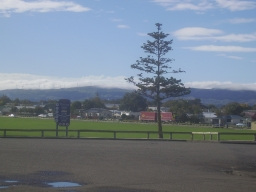
\includegraphics[scale=0.5]{palmerston_n.jpg},]
Marijcke Vlieg was to meet us at the station. The train came in earlier
than the advertised time (but I think later than it was supposed to arrive),
and we managed to get out of the station while she was looking for us on
the platform; but eventually she found us, and took us to the motel, on
the wide and motel-lined Fitzherbert Avenue leading south to the Massey
University campus. They
had our room ready, so we took our bags in. Then Marijcke took us to show
us the campus, and took us back a different way which included a stunning
view of Ruapehu (the mountain seen from the train, which she identified
for us) before dropping us off back at the motel.
\end{window}

The weather was now clear and beautifully warm, so we decided to make use
of the best part of the day and went for a walk in the park and along the
Victoria Esplanade, a lovely park stretching along the bank of the Manawatu
River. We started downstream, dodging the men and machines
laying a big pipeline, and then headed back a bit off the river, through
the native bush. The air was full of birdsong. We heard several tui, but
one in particular sat in a tree just above our heads and serenaded us
for ages with a symphony of chimes, whistles, clicks, rattles and farts,
his body sometimes quivering with the effort of producing the remarkable
selection of sounds. For me, one of the highlights of the trip so far!

\begin{window}[2,r,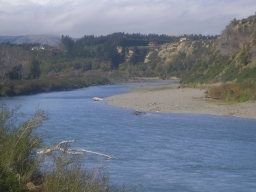
\includegraphics[scale=0.5]{manawatu.jpg},]
It was clear that the native birds preferred the native bush, while thrushes
and huge numbers of blackbirds stuck to the manicured lawns with European
trees including some fine English elms (of course, impossible to see these
in England now).
We walked under the river and up to the cliffs on the other side. We passed
a sign warning us of rock falls from the cliffs, and right on cue, half a
tonne of rock broke away without any warning and tumbled down into the water.
On the flat ground beside the river we found a variety of interesting flowers
including a woody bush with yellow lupin-like flowers.
\end{window}

\begin{window}[1,r,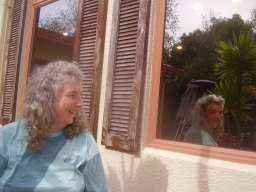
\includegraphics[scale=0.5]{elmcafe.jpg},]
We strolled back to the motel, and decided to try the Elm Caf\'e for lunch.
They were still doing brunch, so we settled for that: the food was a work
of art, both in looks and taste. During and after lunch, the sky became
considerably more cloudy; though still sunny, the morning's sharp clarity
was lost.
Back at the motel we found a note asking me to phone Matt Perlmutter. The
phone in our room wasn't working so I had to get another from the desk.
I walked in to the University in the afternoon to touch base with Matt;
about 3km, no signs but only one path so no chance to go wrong. 
\end{window}

They have
given me an office with no computer, but Matt got an IT person to set me
up so that I can connect the white toy to the  network. I can't use a
web browser, but ssh and scp work fine. Indeed, reading my email I found
news that Adrian Smith has resigned as principal of Queen Mary, and proofs
of the Topology paper with Sam Tarzi to be corrected; I was able to fetch
both of them across without any problem.


I walked home, after finding a different way from the road to the University
(through a little park on the banks of a stream, with many tree ferns). On
the way home I saw a curiously jagged but localised black cloud in the sky
along with all the white clouds.

In the motel I worked for a while. There was a dramatic sunset visible
from the motel balcony. Then we walked towards town for dinner in the
first eating place: it was pleasant enough though we might have done
better in the Elm Tree.

We woke the next morning to pouring rain: the clouds and the amazing suset
clearly presaged a major change. Of course this played havoc with the
morning traffic, and so Rosemary's contact at AgResearch was a few minutes
late. I had intended to walk again, but given the weather I decided to blag
a lift in the back of his tiny car. I walked up to the University through
the little park, and found that the network connection was still working
perfectly (unlike the situation in Christchurch). So I read my email and
sent off the proof corrections to the Topology paper.

After coffee, Rosemary arrived from AgResearch, and it was time for my
talk. Introduced as ``the first Forder lecturer to use public transport'',
and faced with the most technical of all my talks (the one on orbit
counting), to an audience of sixteen, I think I made a reasonable job
of it.  Then we went to lunch in the lovely old homestead, set in a beautiful
garden, which was the original University building. By this time, the rain
had stopped and the sky had brightened a little.

Matt had mentioned, in introducing me, the fact that the eleventh Forder
lecturer should have come in 2007. At lunch, Robert Maclachlan alluded to
happenings behind the scene but didn't encourage discussion. So perhaps
I have misread the signals. I concluded that I really don't know what is
going on.

\begin{window}[1,r,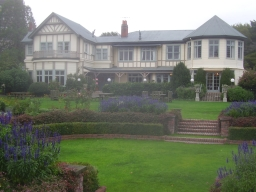
\includegraphics[scale=0.5]{staffclub.jpg},]
After lunch we tested the equipment for tomorrow (which worked perfectly), 
and then I read email again before Rosemary's second talk. After that,
a drink in the Staff Club. (In fact, it used to be the Staff Club, but
the University took it over on some alleged problem about the licence, and
saves money by not opening it all the time, so that often it is impossible
to get a drink after a Friday seminar without driving all the way into town.)
Then we got a lift back to the motel with a statistician. The rain was still
pouring down; we tried the Elm Caf\'e but it was fully booked, so we got
sandwiches in the BP service station and ate them in the motel room.
\end{window}

Next morning the rain had stopped; it was still cloudy (with small patches
of blue) and very humid. I walked to the University, hearing the screaming
of plovers as a harrier wheeled overhead. The river was much higher and
the water very brown. I walked up to the campus through a different but
even more pleasant garden, and discovered that Human Resources meet in a
``tree house'' (really just a house surrounded by trees).

My talk was in a much larger lecture theatre, and about 80 people showed
up, most of them students. (Some of the students had to leave before the
end, presumably to another lecture.) It went well, I think -- there were
no questions afterwards, again probably because they had lectures to get to.

Matt had a meeting, but had planned a trip with Kee Teo and Charles Little,
so he drove us to Charles' car (which he parks in a suburb about a kilometre
from the campus). We went looking for Rosemary, but she wasn't in the motel
and we didn't spot her on Fitzherbert Avenue or in the Square, so we went
without her.

\begin{window}[0,r,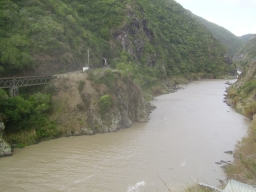
\includegraphics[scale=0.5]{gorge.jpg},]
First we drove through the Manawatu Gorge, where the river has forced its
way through the mountains. Lovely scenery but not as rugged as one might
expect; the rocks round here are very soft. (On the road, there was evidence
of recent rockfalls, the cliffs were covered with wire netting, and men in
orange jackets were at work high over the road replacing the netting on a
recent fall.) On the other side, a railway line (to Hawke's Bay) twisted
in and out of tunnels. It is clearly still used though not for passengers
(except for a few specials).
\end{window}

After that we drove up to the wind farm, where there is a small car park
right under one of the windmills, which swishes away above your head as you
look out. The noise is not too intrusive. Kee resented the way the windmills
intrude on the landscpe, especially poking their heads over the rim of the
gorge; but this seems so much better than a nuclear power station to me.
The wind was quite strong and a shower was passing. (When it cleared later
we could see a patchwork of sunshine and showers on the valley below.) Then
back through Ashhurst to the University.

Charles told me about an idea of his which might throw some new light on
the vexed existence question for Hadamard matrices. He has taken the same
idea I used when Bert was writing his thesis, expressed it in terms of
coding theory, and proposes to use the MacWilliams relations to get some
new information. He gave me a copy of his notes. I will certainly try my
hand at it! In another surprising connection, Matt told me that he is doing
some calculations on root systems which involve thinking of them as matroids.
I mentioned Gary Gordon's name to him and promised to send him Gary's email.

The sun had come out by then, and on a glorious evening I walked back to the
motel, with a detour by the Victoria Esplanade. A tui was singing in a tree,
but I knew it wouldn't match the experience of two days ago, so I walked on.

We were sent off with a delicious and congenial dinner in the Elm Caf\'e.
On the way there, the moon was shining brightly, close to full, and the
Southern Cross, Pointers, Orion and a few other stars were struggling to 
appear behind fitful clouds.

\section{Through the centre}

The next morning dawned beautifully clear, the mountains sharp against
the sky, but with an ominous line of low cloud on the horizon.
After breakfast, Kee came to take us to the station. The train was due
to leave at 9:45 and the official instructions are to arrive 20 minutes
ahead of time, so we had told him 9:00, and he arrived a bit early. So
we were at the station at 9:10. The door was locked. No problem, you just
go round the side. Nobody on the platform. No problem, there are a few
luggage labels on the table in the waiting room, you tag your own bags.
I knew from Wednesday where the baggage wagon would be, and was there long
before the rest of the (quite large number of) passengers getting on had
figured out the place.

Out of Palmerston North, across the plains, through Bunnythorpe (the place
where Glaxo began, according to Charles) and Feilding (the town whose
plan is based on Manchester, looking almost but not totally unlike its
model). Then we went through some low and rounded, mostly treeless, hills.
The other side of the hills we crossed the Rangitikei River, climbed the
other bank, and swung in a huge curve to follow the river.

The river ran in a very deep and steep bed in a wide and flat plain bounded
by hills. Descending the west bank hills, we ran along at their foot, with
views over the plain to the other side. After a while we turned up a pretty
side valley, where we steadily climbed. Back over the hills to the main
valley, which had narrowed down, and which we proceeded to cross and
re-cross several times on huge viaducts more than seventy metres above
the river, with very impressive views of the river and its high cliffs.

\begin{window}[5,r,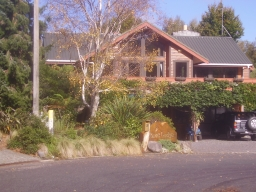
\includegraphics[scale=0.5]{dakune.jpg},]
Again we turned up a side valley passing farms with deer and cattle. We
decided to eat lunch before Ohakune; I had a railway meat pie and a can of
Speights' Old Dark. The train reached high moorland with an army training
centre, and eventually we arrived, just a little late, at Ohakune.
We were the only people to alight from the train, but the staff opened the
doors for us and had our bags ready. And there on the platform was Nicolas
Cowell of the \href{http://www.dakunelodge.co.nz}{Dakune Lodge}. 
He took our bags and loaded them in the big car,
then took us for a drive around the town of Ohakune (which is stretched
between the railway and the main road), pointing out all the walking 
tracks, and finally took us back to his guesthouse and showed us our room.
\end{window}

He invited us to look at the paper. There, in the flannel panel, was a notice
of an article about the eee-pc. He noticed that it caught my eye, and I said
that I had one, which I got out to show him, We tried to connect it to his
wireless network, but something wasn't working right, so we abandoned the
attempt.

We went out for a walk. The weather had got steadily greyer as the train
progressed, and it started raining almost as soon as we left the house
(fortuately only a shower). Of the various options, we decided to walk in
the National Park first. There were two loops, one said to take 15 minutes,
the other an hour. We did both, a little slower than the signs suggested,
partly because of Rosemary's knee, partly because we kept stopping to look
at things.

\begin{window}[2,r,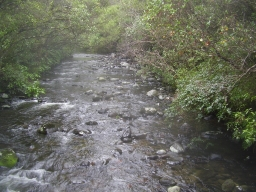
\includegraphics[scale=0.5]{npwalk.jpg},]
The first, short trail was very level (suitable for wheelchairs). The
air was full of lovely birdsong, and a fantail displayed to us from a low
tree. This took us to the start of the second trail, which was a bit less
well maintained. As we climbed, we noticed the air getting much colder,
and the birdsong diminishing to silence, with only the sound of the stream
in its bed and a train passing (presumably the southbound Overlander).
Among the magnificent trees we saw were red and black pines, totara, tawa,
and rimu; there were also many smaller trees such as pepperwood (the sign
saying it grew to 2 metres was by a tree at least twice this height).
I was a bit surprised at the lack of fungi, but at the end of the walk there 
were some, including a spectacular tree fungus and a big red one. We saw a 
New Zealand robin, who serenaded us with his squeaks, and an unidentified 
bird with a forked tail high in a tree who made harsher repetitive squawks.
\end{window}

\begin{window}[7,r,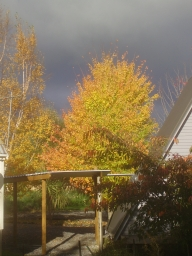
\includegraphics[scale=0.5]{autumn.jpg},]
When we came out of the national park, the display on the road sign was
saying that the road was closed because of snow. Certainly the weather
had turned much colder, but there was no sign of snow or rain where we
were, and breaks in the cloud were allowing sunlight
to play on a distant hill, and eventually on us as well. But it was too
cloudy to see the mountains.
We took the riverside path down to the other part of the town (on the main
road where the shopping centre is). Enough sun came between the clouds to
illuminate the very brightly coloured autumn leaves, often standing out
against the dark clouds. The bank was steeply undercut in any places, with
trees and clumps of pampas grass perched precariously on the edge.
On the other side of the fence was a complete contrast: cattle grazing
country, with ragwort and brambles.
We decided to continue on the Jubilee Walkway, which we managed to find 
despite the inaccuracy of the map (showing it starting on the wrong side of
the river). This was more lovely native bush, more unkempt than in the
National Park, but very atmospheric. We crossed the bridge into the town
centre, checked out possible restaurants, and walked back to the Dakune
Lodge. Rimu Street looked at first a bit like a street in Toowoomba (wide,
grass verge and concrete footpath, red soil, old weatherboard houses),  but
then we got to the new developments including a village of yurts and the
illusion was quite shattered.
\end{window}
Rosemary had walked her quota for the day and wasn't looking forward to
another trip across the town and back. But Nicolas and Tasha offered to
give us a lift down town, so we would only have to walk back. We ate at
the Alpine Restaurant, run by a Austrian who had arrived in New Zealand
in 1973; delicious pumpkin soup, venison and ostrich, and a very nice
Eskdale merlot/cabernet/malbec. Also, the first place I have found so far
in New Zealand to accept a credit card PIN.

Walking back, we found that the night had cleared, apart from fluffy white
clouds over the mountains. The moon was very close to full, and stars blazed
in the sky.

Arriving back, we had  just started writing our diaries when our hosts
also returned. So we tried out the wireless again; this time it worked
without a hitch. So I showed Nicolas the 
\href{http://antwrp.gsfc.nasa.gov/apod/astropix.html}{Astronomy
Picture of the Day},
and 
\href{http://en.wikipedia.org/wiki/Peter_Cameron_%28mathematician%29}{my
Wikipedia page}, from which we followed a few links (to the 
\href{http://en.wikipedia.org/wiki/Erd%C5%91s_number}{Erd\H{o};s
number page}, and to 
\href{http://en.wikipedia.org/wiki/Toowoomba}{Toowoomba}). On the 
Toowoomba page we found a link to
\href{http://terrytao.wordpress.com/about/petition-to-support-maths-statistics-and-computing-at-usq/}{Terry Tao's petition}
against the closure of the mathematics department at USQ. I had been told 
about this but had not had time to look at it
before; now, I decided that the time had come for me to sign it and put
in my comments, which I did.

Next morning we showed up at 8 for the ``continental'' breakfast of cereal,
toast and coffee, quite adequate for our needs. I had persuaded Rosemary
that she had done enough walking and would be better off having a rest
(needless to say I should have saved my breath -- she went out and did the
forest walk from yesterday in the reverse direction),
but that I would walk the old coaching road, which Nicolas had told us
about: before the railway was completed, northbound passengers would
detrain in Ohakune and would be taken by horse-drawn coach to the railhead
on the other line. Just as I was setting off, Nicolas said ``Would you like
company?''

He drove us out along the Old Station Road to the point where the track 
crosses a small stream and goes up the hill. The roads were rather like those
of my youth, dusty and unsealed. The hills in the distance were amazingly
clear.

\begin{window}[2,r,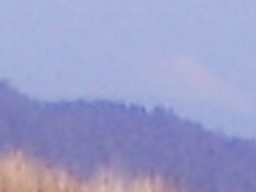
\includegraphics[scale=0.5]{taranaki.jpg},]
A plank bridge crossed the stream. Nicolas said that there are plans to
build a proper bridge, but they have to do it before the trout spawning
season starts, or else they are not allowed to do it until the season
finishes. Trout fishermen trump trampers!
The track went up a hill with fine views over the farmlands to various hills
and mountains at various distances. At a certain point Nicolas stopped to get
his bearings, and then directed my eyes to a certain mountain slope to look
for a white thing. It took me a few seconds to see, ghostly and far far
beyond the line of mountains, the symmetrical white shape of Taranaki standing
up into the sky. Another of the most amazing experiences of the trip. (The
photo doesn't do it justice though!)
\end{window}

This was a lovely walk altogether, full of interest. At a certain point
Nicolas stopped to show me a lancewood tree, trunk as straight and thin as
a curtain pole, sharp rough leaves pointing straight down. He told me to wait
until we rounded a corner. There was an apparently quite different tree, with
a thicker trunk completely bare of leaves and a crown of more normal leaves
above our head. A mature lancewood. This, it seems, was their strategy for
dealing with predation by moas. There is not a shadow of doubt, since around
the mature lancewood were some younger ones in the form we had seen. We also
saw a small black bird with white on its front, probably a tom tit.

\begin{window}[3,r,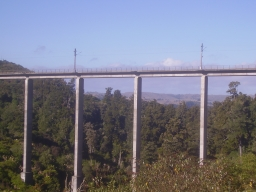
\includegraphics[scale=0.5]{viaduct.jpg},]
The track left the old coach road -- this crosses the line of the railway and
the company do not permit its use. We descended on a well-made new trail
(but steeper than the coach road, which had to have no gradient steeper than
a horse-drawn coach could manage). We came to a tunnel, used by the railway
before it was re-aligned some years ago. It is possible to walk into the
tunnel, and possibly out the other end; but this is discouraged because it
debouches directly onto the existing railway track (they sliced right through
the tunnel making a new cutting).
Following on, we came to the two huge viaducts, the old iron one, and the
new concrete one on a curve, with spectacular views of both, and beyond down
the valley and out onto the plain. Then up the hill on the other side, through
the old quarry (closed after a blasting accident), past the old house of the
Chinese family who were the first market gardeners (Ohakune now has a giant
carrot, which we didn't manage to see(!)), and back to town. 
\end{window}

As we passed the station, the snow-covered slopes of Ruapehu were visible,
though the summit was still shrouded in cloud. Nicolas took
me back to the guesthouse a different way, round the backs of the houses in
Park Avenue where there are a couple of lakes being restored by private
enterprise.

Apropos of the missed opportunities for train travel, including the rather
stilted commentaries, Nicolas told me about a car junkyard (which we later
saw from the train), which is world famous as a source of spare parts for
old cars unotainable elsewhere. In return I was able to tell him about
Glaxo and Bunnythorpe.

His friend, a house painter, was in the kitchen, and they had coffee and cake,
and offered me one on the house (despite the notice on the wall giving the 
charges for things like this). I picked up a magazine on the hearth:
\textit{Lifestyle Farmer}, with articles like ``How to tell if your alpaca is
pregnant'' (if she spits at the male, she is!)

Then Tasha drove Nicolas to fetch the car, 
after which Nicolas took us to the station. There were two people on the
platform already, waiting to pick up somebody arriving by train; they 
started in on a rant about the disgraceful state of New Zealand railways 
even before Nicolas had gone. By now the clouds had cleared and the whole of
Ruapehu was visible. What a lucky choice we made with Ohakune as a
stopping place!

\begin{window}[1,r,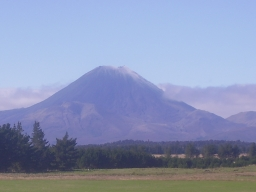
\includegraphics[scale=0.5]{tongariro.jpg},]
The first leg was the short journey to National Park, the lunch stop. On
the way we crossed the viaduct I'd seen that morning and a couple of others,
and had some spectacular views of Ruapehu, the top covered in snow. Approaching
National Park, Tongariro came into view as well. When we arrived, most people
headed for the caf\'e but we thought it much better to join the very few 
hardy souls who walked through the little town to get a view of the mighty 
mountains unimpeded by overhead power lines, street lights, etc.
\end{window}

Shortly after leaving National Park, we came to the Raurimu Spiral, of which
they are very proud. As we went round the spiral and the horseshoe bend, the
conductor drew our attention to bits of track we had passed over or were about
to pass over, much higher or lower on the slope. From one point, all three
lines were visible. After this excitement, the buffet opened and I went to get
lunch.

Down from the mountains, the country was much gentler. We went down the
Whakapapa River, a tributary of the Whanganui, and then the Whanganui itself,
and then turned up another tributary, the Ongaruhe. The valley became
narrower, the strangely-shaped hills more rugged, and finally we left the
river and after a short distance up a side valley plunged into a tunnel,
emerging in the Waikato catchment. Now the scenery played out in reverse
as similar-shaped hills receded and became less rugged and eventually we
came to flat open ground. After the hills, cirrus clouds appeared in the
sky beyond the small fluffy cumulus; who knows what change they presage?

\section{Hamilton}

At this point the driver put his foot down and we rattled along at what
seemed like a great rate, spilling our coffee over ourselves, and arrived
in Hamilton half an hour early, so that Ernie Kalnins, who was meeting us,
was caught out and came while we were standing on the platform with our
luggage. He took us to the motel to check in, and then whisked us off to
a lovely relaxing evening at his house eating a delicious lasagne that his
wife Anne had cooked. (Getting to the motel was a bit tedious since the V8
races, which had been on all weekend, had just finished and everyone was
heading home very noisily.)

Then the coincidences began. Anne had grown up in Garston Manor, when it was
a hospital (now it does wedding receptions including James' and Debbie's);
her mother might have delivered Rosemary. She showed me an old photo of
the manor house and a painting of the countryside at Bricketts Wood, including
what is unmistakably an elm tree.

More talk about the future of the Forder lectureship. Could it be updated
in the way that the LMS has done with the Hardy lectureship, having the
lecturer based in one place and making trips elsewhere? Or combined with
something like the Erskine fellowships in Christchurch?

Next morning, breakkfast at Zigi's. (Rosemary had stayed here a few years
ago and knew the best breakfast spot!) On the way we were surprised to see
several camellias in flower, despite the season being mid-autumn. We put 
the laundry on before breakfast, and had it finished and dried (after a
fashion) before Kevin Broughan came to collect us.

Walking back from breakfast, we spotted a little bird high in a dead tree.
I was looking it up in the book (it was a grey warbler, I think), when a
car with three youths in it pulled up beside us. ``Excuse me, mister'', said
one of them, ``are you a published author?'' ``Yes, and so is she,'' I replied.
(Rosemary's book came out just before we left and she brought a copy to
show to statiticians on this journey.) In Hamilton we also identified
silvereye and mynah birds.

\begin{window}[2,r,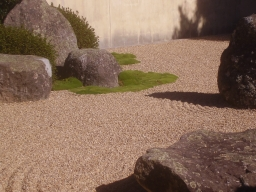
\includegraphics[scale=0.5]{zengarden.jpg},]
We started with a trip to \href{http://www.hamiltongardens.co.nz/}{Hamilton
Gardens}, and a walk round the Paradise
Gardens, six small but beautifully executed gardens in various national
styles: Italian Renaissance, Indian Mughal, Chinese scholar's garden (with
a very dense bamboo grove), English (the weakest of the lot, I thought), 
American modernist (with a screenprint of Marilyn Monroe)
and a Japanese Zen garden with raked
stones, mossy boulders, and a lovely dwarf maple tree. The gardens backed
onto the Waikato River; from one of the terraces, we saw a kingfisher.
The Italian garden included a small classical amphitheatre that would be a 
splendid setting for chamber music or an intimate play.
\end{window}

Then we went to the university, were given an office, and went to coffee,
in the common room with lovely views over the sunlit campus and to the
northern mountains.
There was only a small time gap between coffee and lunch, but Kevin managed to
tell me a few very interesting problems about factorials modulo a prime.
At lunch quite a few other people joined us, sitting on a shady terrace.
Then Kevin took me to a cash machine. On the way, we met the Vice-Chancellor
(who admitted to having contacts in the Materials department at Queen Mary).
Back to the Mathematics department, and Kevin went to sort out the lecture
room.

It had cables all over the place, some of them connected to nothing, others
to who knows what; some power points working, others not; no way to turn on
the data projector except by standing on tiptoe; and in the end the system
refused to respond to the white toy. The technicians tried to blame my 
computer, but in a room as disorganised as that, I know what the more likely
source of trouble was. I found later that even the power socket on the 
lectern wasn't live, so the batteries on the white toy had run down somewhat.

But no worry, Kevin found another room (much nicer, with a high ceiling and
more seats), checked that the equipment worked, and went away to put up
notices directing the audience to the new location.

The two back-to-back talks (mine on Sudoku and Rosemary's on row-column
designs) went well, and even had some ideas in common. There were 23 people
at my talk, slightly fewer at hers. Several good questions at both talk.

\begin{window}[1,r,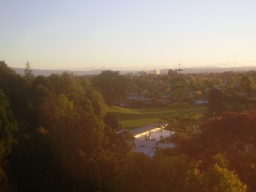
\includegraphics[scale=0.5]{hamilton.jpg},]
Afterwards we had wine and nibbles in the tea room with its stunning view, 
and watched the sun set, the light fade, and the huge moon rise in the clear
sky. We were in the hands of the statisticians, who took us to the Domaine,
a very good restaurant down town where I had venison followed by passionfruit
creme brulee, with a Hawkes Bay merlot/malbec. (Our first choice had been
a French wine, a Cotes de Ventoux, and it was remarked that the French have
been forced into varietal labelling -- it was a grenache/syrah -- but sad
to say it was unavailable; the restaurant are in process of changing their
wine list and were running down their stocks.)
\end{window}

\begin{window}[2,r,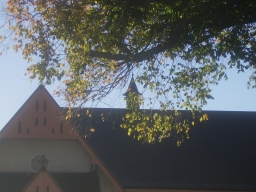
\includegraphics[scale=0.5]{zigis.jpg},]
After dinner we were taken on a detour to see the V8 racing course through
the centre of town: the stands and barriers not yet demolished, and piles
of wrecked cars waiting to be taken away.
Next morning, on the way to breakfast, we saw a traffic jam with the rush
hour traffic being re-routed by police. It turned out that a car had run
into the back of a bus just up ahead. By the time we finished breakfast,
they had cleared it away and got traffic flowing again. The sky was clear
and another nice day seemed in the offing.
\end{window}

Kevin arrived and took Rosemary in to town to go to the museum. Just as we
let her out, the rain started coming down in buckets. Kevin said, ``By the time
we get to the University it will have stopped'', and he was almost right. It
did rain several more times but with nothing like the vehemence of this
downpour.

I read my email, which included one from Eamonn (about an interview for the
Kim Hill show on Radio New Zealand while I am in Auckland), one from Marie
telling me that New Zealand was having a serious drought (I was able to update
her on that), and one from Harold about Wayne Gould, the New Zealander who
introduced the world to Sudoku, along with two things to read from students
which after some difficulty I emailed to Kevin who printed them out. We had
lunch (indoors, as it was drizzling), and I had a long talk with Kevin about
various mathematical topics, including Lehmer's conjecture and a variant, and
some of the work we have done at the Newton Institute about chromatic roots
from the viewpoint of algebraic number theory.

Then it was time for my talk on ``The Random Graph'', once again in the nice 
room on the third floor. It went down very well and provoked a lot of
discussion, both in questions after the lecture and at refreshments afterwards.

We went to Cullen's for dinner, where I had tuna coated with black and
white sesame seeds (so tender that it was easy to cut with chopsticks),
with dipping sauces and tempura vegetables. We had a bottle of pinot
gris from Hawke's Bay. Kevin said that one suggestion I had made to him
(that the case $n=4$ might be easier than $n=3$) seemed to have
been a good one.

\section{Interlude in Northland}

Next morning we walked to Zigi's for breakfast and found it in some disarray.
I think the chef hadn't turned up; it was almost an hour after our arrival
when the food finally came. Rosemary was getting a bit nervous as she had
left her packing until after breakfast. But it finally came together, we
were ready a minute before Ernie arrived to take us to the bus station.

Apart from trying to board the Wellington bus by mistake (none of the buses
are labelled and there are no set stops), we got away all right, though
rather late. But the driver didn't exactly inspire confidence. He hit the
kerb turning onto the expressway, and nearly got us squashed by a big truck
that wouldn't let us off the slip road. After the bus had laboriously hauled
its way up the hill out of the Waikato valley, the driver remembered that he
had forgotten to let someone off, so he had to turn off, cross the
expressway, drive all the way down the hill, turn round in a deserted service
station, let the passenger off, and struggle back up the hill. (He had
probably forgotten because he was deep in conversation with a passenger
sitting behind him, not concentrating on his driving. At one point, in
answer to a question, he said that he had been driving the route for
thirty-five years.) Then at Manukau, he drove away with one disembarking
passenger's luggage; she had to bang on the side of the bus to get him to stop.

It was not such an interesting journey as some we'd had. Flat plains of
the Waikato, with a few small hills (the first ones the river had burst 
through, the next it detoured around), until we left it for good. A much 
grander river than any other we've seen here, wide and full. Then mostly
suburban from there into Auckland. After the various adventures, the bus
was nearly three quarters of an hour late, but we had time for a toilet
stop and some sandwiches before the Northland bus came.

This bus was also late, though more through a comedy of errors than
incompetence, I think. The refuelling stop in Albany involved a lot of
pointless driving up and down the same road. The driver was a bit slow
getting us back on the bus after the refreshment stop. Then he drove all
the way to the other side of the village of Kawakawa to drop off a boy,
and all the way back, only to find that his parents were waiting in a small
park just off the main road.

\begin{window}[4,r,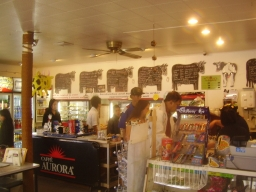
\includegraphics[scale=0.5]{swingingcow.jpg},]
This was a very scenic stretch, once we were out of the tedious Auckland
suburbs. At Orewa, and for the next little while, we had abrupt cliffs
sheltering tiny beaches, islands out to sea, and green hills behind. There
were a couple of estuaries, with wide mudflats, some covered with mangroves.
Then we left the coast and headed over rugged hills. We came down to touch
the ends of various inlets from Kaipara Harbour on the west coast.
The refreshment stop, halfway up a very long climb, was at the 
Swinging Cow caf\'e. It took its name
and its theme from a clock whose face was in the shape of a cow, the cow's
udder being the pendulum. All the decor, menu boards and gimmicks for sale,
seemed to be cow-themed. We were not hungry so strolled around outside until
it was time to go.
\end{window}

From the top of this hill we had a splendid view of Northland: blue sea and
headlands and islands, green grass, shining brilliantly in the westering sun,
with the burnished leaves of the trees. A magical vision, which we then
descended into. We touched the beach, crossed some more hills, went through
extensive mangrove swamps on inlets from Whangarai Harbour, and finally into
the town of Whangarai. Because of the delay, we were caught in the town's
appalling rush hour traffic, but finally we escaped onto the open road.
A steep ascent and a long descent into the valley of the Otiria River.
The sun was behind a cloud full of holes, and crepuscular rays poured out
in all directions. 

After Kawakawa, it was too dark to see anything much. We disembarked at the
pier and walked back to the Paihia Star Motel, which we had spotted coming
into town.

After checking in, we dined at the Swiss Caf\'e, and bought breakfast at a
convenience store on the way home.

\begin{window}[1,r,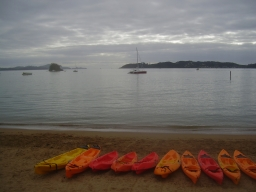
\includegraphics[scale=0.5]{paihia.jpg},]
Next morning, we were woken by an unidentified bird singing descending 
fifths.  After a rather late start, we walked back to the Maritime Building
at the pier. The girl at the Fuller's desk in the entrance managed
to persuade us to buy tickets for the all-day cruise on Saturday, and then
sold us ferry tickets to Russell. She shouldn't have done this -- there are
ferries run by several different companies and the tickets are not
interchangeable, so the correct method is to go down to the end of the
jetty and buy a ticket on the ferry about to leave. In our case this
happened to be a different company, but the Fuller's all-day cruise was
just about to leave, and agreed to take us across to Russell.
\end{window}

We walked along the sea-front at Russell, while the clouds cleared a bit and
the sun came out, and went into the tourist information centre for a map. The
town had a sub-tropical feel to it, with lots of bougainvillea, hibiscus, 
morning glory, and many other bright flowers. We decided to look at 
Pompallier and the museum, then buy lunch and take it to Long Beach.

\begin{window}[2,r,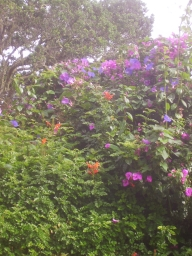
\includegraphics[scale=0.5]{russell.jpg},]
We paid our entrance fee for Pompallier, the old Catholic mission: my
National Trust card would have got me in free but I couldn't find it. Just
as we walked through the gate, we were entranced by some glorious Polynesian
singing, a soloist answered by a chorus in close harmony. It turned out to
be a party of Fijians who were just finishing a guided tour, and had burst
into song. The third highlight of the trip!
The building had been used for printing Bibles and sacred texts translated
into Maori, and there were interactive displays showing how the printing
was done and how the leather for the bindings was made. There was also a
lovely colonial garden from a later phase, including an orchard where the
ripe fruit was providing a feast for a pair of silvereyes. The sun was coming
out, and the colour of the flowers were brilliant.
\end{window}

\begin{window}[2,r,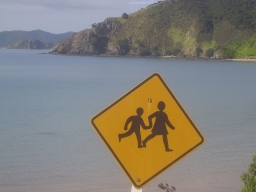
\includegraphics[scale=0.5]{longbeach.jpg},]
We bought a book about the New Zealand wars, and went to the museum, where
pride of place was taken by a one-fifth size model of the ``Endeavour''. (On
his first voyage, Cook spent some time in the Bay of Islands.) The rest of
the exhibition was a varied and slightly motley collection of guns, Maori
weapons and artefacts, a huge crayfish, whalebones, sharks' jaws, etc.
We bought the last two sandwiches and Bundaberg ginger beer in the supermarket
and walked over to Long Beach on the other side of the peninsula to eat it.
A lovely secluded beach with stunning views to vistas of further islands and
peninsulas, where we sat in glorious sunshine eating it.
\end{window}

We agreed to take the fourth historical trail on the museum's list, which
would take us to Okiato, then catch the car ferry to Opua and walk
the Pahia-Opua walkway home. Unfortunately the historical trail was almost
entirely on the main road, with no footpath. There were a couple of steep
climbs where it went over headlands, but for a long stretch it went
round Uruti and Orongo Bays, with lots of mangrove flats. Out to sea beyond
the mangroves in Orongo Bay was an oyster farm. We saw herons on the mudflat
between us and the oyster farm, stilts and oystercatchers, and a pair of
kingfishers who perched on a power line and kept flying on just a bit
ahead of us. About here we found a nice graded path off the road, just
above the mangroves.

\begin{window}[2,r,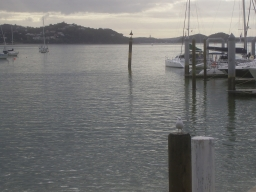
\includegraphics[scale=0.5]{opua.jpg},]
Eventually we took a turn, hoping it would be the Okiato Walkway. It wasn't,
but led us to the walkway, a steep path going up and down to creeks in the
forest, with some of the trees labelled (one a kauri, one a mature lancewood).
The air was full of birdsong, and we saw som good fungi including a huge
round one a long way off the path.  We went slower than we should have, and
decided to skip the site of the original government in Okiato and press on
to the ferry. For a dollar each, we were taken over to Opua.
\end{window}

From the ferry, we saw a tern fall to the water like a stone after a catch,
and then a larger bird (which looked like a gull but I think must have been
a gannet) doing a power dive into the water with wings tucked in.

We found a bar and sat on the verandah; when a man came, we asked for tea, 
which he agreed to bring. It took a long time, and eventually he brought it
with an apology for the delay, and said that in fact the bar was closed from
three to five, and that because of this he wouldn't charge us for the tea!

We went to look for railway rolling-stock on the old line, but it has all
been converted into a mammoth marina with rows and rows of yachts; so we
eventually set off for Paihia.

It was a delightful path, following the coast. Sometimes the path was cut 
out of the soft cliff rock, just above sea level; sometimes it went higher
on the cliffs through lovely native bush, with many tree ferns at the lower
levels; sometimes it descended to tiny secluded coves, some with camping
sites, some completely deserted; and at the Waimangaro River crossing, it 
took us on a long boardwalk through the mangroves. The light was beginning
to fade, and the reflections in the calm waters of the Veronica Channel were
really lovely. But the steep narrow paths on cliff edges were taking their toll
of Rosemary, and after crossing over the Haumi River bridge, she decided to
walk on the road back to Paihia. In the gathering gloom, I took to the beach.

It was all easily negotiable, or would have been if the light had been better.
I had to scramble over some rocks; at one point, I nearly walked into a
rock pool, mistaking it for a patch of sand; at the end of the path, I
nearly walked into a chain put up to keep cars out. But eventually I was
back, arriving at the motel almost exactly simultaneously with Rosemary.

In the end, the maps were not a lot of help to us. Both the Northland map
(which included an enlargement of the Bay of Islands) and the 1:50000 map
by the Land Information Department were inaccurate about the Okiato Walkway;
we only got accurate information from a girl jogging the trail who passed us.
The Land Information map didn't show that Paihia - Opua Walkway, and the
other map showed it as hugging the coast very closely, so I had inferred
that no climbing would be required.

After a shower and change, we went out to eat. Number 6 was open, and we
went in. I had a very tasty whiting in cream and white wine sauce, with
garlic bread and half a litre of Bavarian weissbier. The proprietor, a German,
came out to talk to us.

Next morning, the same bird was our alarm clock. After breakfast we headed 
for Waitangi, stopping to take a look at Te Tii (a complex including a Maori
meeting house and looking rather like a school) and the Sugar Boat (once a
restaurant and now for sale and looking very decrepit). We began the 
Waitangi trip with a coffee in the Waikokopu Caf\'e. We watched eels 
swimming in the pond, while a small boy fed the ducks under a sign saying 
``Please don't feed the ducks'', and his family did nothing to restrain him, 
except for saying ``No more'' when he wanted another scone.

\begin{window}[1,r,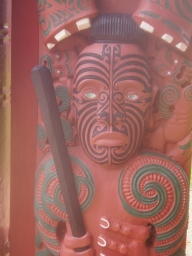
\includegraphics[scale=0.5]{waka.jpg},]
We paid the entrance fee to the site. (It is fenced off from the car park
and the caf\'e; we found later that you can walk through it on the coastal
path, but if so you are not supposed to stop and look at things.) We
saw the ceremonial waka (war canoe), specially made from three kauri trees
for the centenary of the treaty, and elaborately carved. 
Next was the
Treaty House, actually the home of James Busby, the British residennt from
1833 (the treaty was signed on the lawn in front of the house). He was
sent from Sydney, as was his house (prefabricated of bluegum); the size of
the house was cut down on the Governor's orders on the grounds of expense
(he had only two bedrooms for his large and growing family), and he was
given very little support, no troops or police, and expected to keep
order with Kororareka (the ``hell-hole of the Pacific'') just across the
bay and Maori settled densely around. The fact that he was so well thought of
despite all this says a lot for him. He helped the new Governor, William
Hobson, draft the treaty (presumably steering him away from what would be
unacceptable to the Maori chiefs). One of the most revealing documents was
his address to the chiefs on arrival, in which he explains that England used
to be as New Zealand is now, a patchwork of warring clans with no decent
clothes or housing -- but look at us now, you too can be like this if you
accept our religion and civilisation! We saw the Whare Runga (meeting house)
built adjacent to the Treaty House, and the ancient and huge camellia trees
planted by Agnes Busby. Then we went back to the caf\'e for lunch.
\end{window}

\begin{window}[1,r,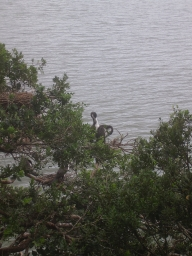
\includegraphics[scale=0.5]{shags.jpg},]
After lunch we walked the trail to Haruru Falls. This was a very nice path,
certainly the best maintained we've found in the Bay of Islands. Crossing
the golf course, we went into a long stretch of native bush, alternating
between fern trees at low level and the more common sort higher up the slope.
At one point we were level with the top branches of a tree in which there
were several cormorants' nests, and adults feeding juveniles.
Then the path descended to a boardwalk through the mangroves. The whole
mangrove forest was talking to us in clicks and pops. (According to the
information board, these sounds are produced by snapping shrimps.) A
mangrove swamp is as productive as high-quality farmland, but because the
people who reap the rewards (the fishermen) are not the same as the owners
of the land, the mangroves are under threat. The solitude, shapes and colours
of mangroves have always appealed to me.
\end{window}

After a long low-lying section near the estuary, we climbed again and came
out to the falls, broad rather than high but with a very impressive flow
of water coming over.

\begin{window}[1,r,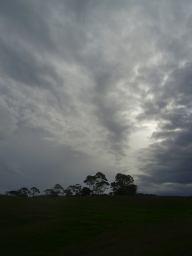
\includegraphics[scale=0.5]{sky.jpg},]
I had decided to walk up to the Paihia to Kerikeri track and back along that,
and persuaded Rosemary that it was little further and would be possible for
her too. In fact, in spite of the trail being clearly shown on the map, 
the walk was entirely along the unsealed gravel road. There was not much
traffic, and many of the cars slowed down to pass us, though not all did!
It was a very pleasant country road, with numerous views over bay, inlets, 
mountains, and green farming country. There was some forestry by the roadside,
but some native bush. We saw a red flowering gum, and a tree with pinnate
leaves and lilac flowers shaped like bean flowers.
\end{window}

Coming back to the golf course, I wanted to take the coastal path, and again
Rosemary came with me. At first there was no path at all, and we had
to follow the edge of the golf course, aboge a ravine in which a bird with
an astonishing metallic edge to its notes sang to us. Then a faint path
began along the edge of the low cliffs, through old trees and flax, finally
bringing us to the edge of the Treaty House lawn, past the war canoe, and to
a booatyard, where we had to wend our way through as the path was nonexistent.

We ate at a Chinese restaurant and bought juice and fruit for breakfast on
the way home.

\begin{window}[0,r,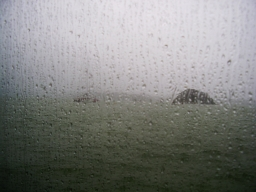
\includegraphics[scale=0.5]{rain.jpg},]
Next morning, it was raining steadily, and as we walked to the pier we
could see that the waves were much bigger than they'd been the last couple
of days. Only eleven passengers boarded the boat for the 
\href{http://www.fboi.co.nz/tour3.php}{Cream Trip}, and when the captain
announced that we were almost certainly not going to be able to get to the
Hole in the Rock because conditions were too bad, two of them left. 
\end{window}

But it was a very good way to spend a wet day, in the hands of our captain 
Hugh, who gave us a very knowledgeable commentary, and his assistant Grace.
Among other things, he gave us a sense of what we might have seen at
different times of year: the red-flowering pohutukawa all around the bay
at Christmas, and the seabirds nesting on the basalt Black Rocks in the
summer.

\begin{window}[1,r,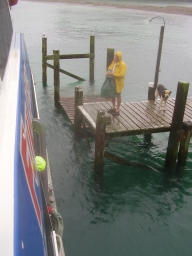
\includegraphics[scale=0.5]{maildrop.jpg},]
In the morning, we cruised around many islands, doing mail and supplies drops
at some of them. It was a little difficult to distinguish between islands with
names like Moturoa, Moturua, and Motuarohia. The Land Information map appends
``Island'' to all these names, which given that ``motu'' means ``island'', 
is a bit
like multiple versions of Torpenhow Hill. At most of the drops, a man (often
accompanied by a dog, who was always given a biscuit) came to meet the boat
and exchange mailbags or take the cartons; but one place had a bucket which
could be hauled in by a rope, into which Grace put a newspaper (wrapped in
plastic, I trust!).
\end{window}

The islands were mostly Government-owned parks, but some pieces were privately
owned, sometimes by millionaires, in one case (Moturoa) by a co-operative
who farmed it. (This island was close enough to the mainland to get its
electricity by overhead cable, under which we sailed.) They were partly
covered by native bush, and partly pasture (in some cases because they were
being farmed, in others because sheep are used to keep the grass down until
the area can be put back to bush). Rocky headlands, eroded by the sea to
cracks, holes and caves, alternated with secluded beaches, one called
Honeymoon Cove because at high tide there is only room for two people.
Some of the coves held expensive houses: one man, unable to obtain
permission to build his own jetty, had tunnelled through the headland so
he could use his neigbour's jetty.

We saw several gannets, flying or sitting on the water -- the captain even
went back to show us one, and persuade it to take off -- and later one
dived on the other side of the boat so we didn't see it. There were also
oystercatchers (both dark and pied) and various gulls, along with many
cormorants, including a very impressive tree full of them.

The dash across the open sea from the northern to the southern islands was
quite rough, and I think everyone understood then why we were not going to
Cape Brett. We stopped for lunch at Zane Grey's resort, founded by the
famous author of westerns for the marlin and shark fishing, and had 
excellent fresh fish and chips. The alternative was a walk up to a viewpoint,
which I was glad not to have taken, when the rain came bucketing down halfway
through lunch.

After lunch, we got to go into the yellow submersible used for viewing fish,
and the captain brought a few fish to the observation windows by tipping fish
food from a bucket. Then on with the voyage; the trip to the cape replaced
by more pottering among the islands and mainland capes and bays. Gruesome
stories of the massacre and cannibalism of the French captain Marion du Fresne
and his crew by Maori -- we learned that, before leaving, the survivors
buried a bottle containing a document claiming New Zealand for France, which
has never been found, and would not be valid since Cook beat them to it --
and the killing of the Roberton family and others by the first Maori to be
hanged under British law.

\begin{window}[4,r,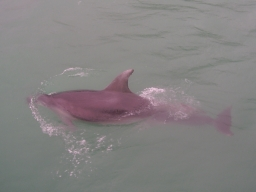
\includegraphics[scale=0.5]{dolphin.jpg},]
The captain explained that the voyage was called the Cream Trip because, as
well as mail and groceries, the Fullers boat used to pick up cans of cream from
the island farms and take them to Opua to load on the train. He was in the
middle of explaining to us that we had arrived at Cream Point, one of the
pick-up points, when he spotted dolphins. He is not allowed to go out of his
way looking for them, but if he finds them he is allowed to take the
passengers among them.
As we came closer, the dolphins put on an astonishing show. They were fishing,
so groups of them would curve gracefully out of the water together; but once
they had an audience, they came over and swam with the boat, and some leapt 
out of the water. There may have been fifty of them altogether, and we were
in the thick of the pod for ten minutes before a dolphin cruise boat approached
and we had to leave them to it. Swimming with them would not have been allowed
since there was a baby in the pod, so we had as good a display as anyone could
have done.
\end{window}

Then there was not much to do but to head home, past two places we visited
in the last couple of days (Long Beach and Waitangi), and back to the motel
for a nice cup of tea. We dined at Only Seafood; I had snapper in banana
cream sauce, with a delicious fruity Gewurztraminer from Gisborne. The
pudding was a bit of a let-down. New Zealand claims the invention of
pavlova, but they really don't understand how to make it: a meringue filled
with cream and floating in stewed berries doth not a pavlova make! No surprise
then that Pavlova didn't make it to New Zealand. In their
favour, they played Beatles songs throughout the whole meal, but so
unobtrusively, and with such competition from the wind and rain outside,
that sometimes it took me several bars to recognise the song. When I was
paying the bill, they were playing ``Yellow Submarine'', which by association
of ideas from today's trip made Rosemary think that we had had this part of
the tape before.

The next morning, the bird had added something to his song: after several
descending fifths, there were a few other notes and then some harsher noises.
I tried to see him but the bathroom window wouldn't open far enough for me
to look out. Later, we saw a tui swelling up as if to begin to sing, then
heard the descending fifths; he was too far away to tell for sure. But even
if he was, he might have just been mimicking another bird. The same song
was coming from all over town. I guess it will just have to remain a mystery.

\begin{window}[0,r,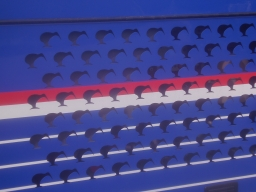
\includegraphics[scale=0.5]{bus.jpg},]
We checked out, took our luggage to the pier where we could leave it, and
decided to walk up to the lookout. The map showed two paths, leaving from
different streets. We tried one, only to find no path and a ``Private Property''
sign. As we walked back to try the other, it started to rain, and we just 
about gave up on it; but the rain stopped and we took the other path.
\end{window}

The path started along a swampy stream, partly on a boardwalk over the stream
itself, and partly along its banks, with a couple of crossings. After the
rain, the sun struggled out and gave the bush the feel of steamy rainforest,
with lots of fern trees. After a while we began to climb; the air grew
cooler, the vegetation changed, with an irregular pine-like tree I couldn't
identify predominating but with lots of celery pine and manuka, as well as
lancewood (both juvenile and adult) and the occasional rimu and others,
and the air was filled with fluting birdsong. Climbing higher, we had
views inland to forested ranges and valleys, and finally a spectacular
view over the bay, with sun shining intermittently on the sea as boats
plied the water and hills rose behind hills. In the distance, the open
ocean sparkled in the light.

Returning to town, we had a coffee, bought lunch at a supermarket, and sat
on a seat in the sunshine behind the lovely old library building to eat it,
then went to catch the bus.

\section{Auckland}

A big bus was waiting; it turned out to be ours, though not yet ready to
board, so we had a short wait. But we got away expeditiously.

We left with blue sky and white clouds; the pastures was a surreal shade
of bright green, with darker green of forests and mountains fading to blue
in the distance. But while we had entered Northland to a wonderful view over
land and sea, this was denied us on leaving; a cloud shrouded the tops of
the mountains and the road ascended into it. Over the summit, the 
cloud disappeared and we had good views over the more settled landscape of
Auckland province.

Later, further and more ominous clouds came down on the hilltops. Coming into
Auckland, these produced a spectacular chiaroscuro through which we travelled.
The tall buildings of Auckland were wreathed in cloud, but the Sky Tower
stood up above the cloud layer into the sunshine. We arrived at the bus
station under the tower five minutes early.

Then we ran into a spot of bother. There was nobody to meet us, so we took
a taxi to the Quadrant. I had a bit of a shock entering the lobby: it sported
a pink motor scooter and fairly loud disco music, and nobody (including the
manager and desk clerks) seemed to be over 25. When I tried to check in,
it was clear that something was wrong. The clerk dithered for a while and
then said he would just go and get the manager ``to take your details''. After
some time the manager came and explained that, because of circumstances
beyond their control, we were unable to stay in the Quadrant, but they had
put us in their sister hotel, the Westin, near the docks. But the point of
the Quadrant was so that I could walk to the University, I explained. Can I
walk from this other hotel? No, it is impossible. But it is not far. How far?
Twenty minutes' walk. We will get a taxi to take you to the hotel, and I will
give you a voucher.

The taxi took a very long time to come. When it did, the driver helpfully 
tried to point out other hotels where we could stay. But we got there, and
they did have a room for us (on the side away from the sea view). 

First impressions were not good. The hotel had a laundry service. They
charged four dollars for a handkerchief, and proportionately more for
other garments. We were looking at a laundry bill of well over a hundred
dollars, as opposed to less than five dollars in the various motels we
have stayed with along the way. I looked up eating places in the Rough Guide
and headed in the most likely direction. Apart from a huge Chinese restaurant
under a car park, the first place we came to was a ``Irish Pub'', which had
the traditional Irish dish Shepherd's Pie on offer, and didn't admit to
selling New Zealand beer until we asked them outright. On the way we saw
paving stones in which the shells in the concrete were still clearly
visible.

The hotel had broadband (of course not cheap), so I read my email, thinking
that maybe someone had sent me an urgent message while we were in the Bay
of Islands. Not a thing.

\begin{window}[0,r,\includegraphics[scale=0.5]{view.jpg},]
My temper wasn't improved the following morning. The room looks out on ugly
office blocks and a huge car park. The breakfast would have been
OK for someone who simply wanted to tuck in and not eat again until next
morning, but for reasonable humans it was far too expensive. They were
also stingy with coffee. Also, breakfast is on a dockside disfigured by
almost featureless apartments (which might actually have been better if they
had been completely featureless). 
\end{window}

\begin{window}[0,r,\includegraphics[scale=0.5]{sign.jpg},]
Setting out on the most direct route to
the University, it took us seven minutes to cross the first road -- crossing
directly was not permitted, one had to go round three sides of a square, one
of which was broken into two stages, and the traffic lights were terribly
slow. The park just beyond the crossing was fenced off from pedestrians with
heavy-duty netting. Not a bird to be seen apart from ubiquitous sparrows.
This is one of the ugliest, most pedestrian-unfriendly cities I have ever
visited!
I found later a sign which sums up the Aucklanders' view of pedestrians.
\end{window}

But at the University, things began to look up. We were given coffee, keys
to an office, coffee, chocolatee biscuits, and a computer account which
actually allowed me to use the computer (unlike other places along the way).
Garry Tee dropped in and presented me with a copy of the book of essays
presented to Henry George Forder in 1970 (which Gaven Martin had shown me)
and an OHP slide made from a scan of his portrait -- a very nice gesture.
The book is:
\begin{quote}
J. C. Butcher (ed.), \textit{A Spectrum of Mathematics: Essays Presented to
H. G. Forder}, Auckland and Oxford, 1971.
\end{quote}

Marston Conder invited us to lunch. And I managed to find time to prepare 
today's talk. 

During the morning, Sepideh Stewart (the occupant of the office we had 
appropriated) came by to collect some things. I had guessed from looking
at the books that she worked in mathematical education; she has just submitted
her thesis but hasn't been examined yet, but she said that she feels the
need for more mathematical knowledge and is thinking of enrolling for some
more maths.

Also, it was pointed out that in the 
\href{http://www.nzherald.co.nz}{\emph{New Zealand Herald}},
right under the easy sudoku, there was an advertisement for my public lecture! 
We couldn't steal the paper then since the mathematicians solve the sudoku 
and cryptic crossword over lunch and someone has to copy them; but I managed 
to make off with it in the afternoon.

Marston took us to lunch at a nice Japanese restaurant (run by Koreans, as
apparently most of them are!), and then coffee in the students' union 
caf\'e (grandly known as the Relax Lounge),
and then it was time for my talk. This was the one on ``Cores, hulls, and
synchronization''; as usual, too much material, but I think I did a fair job.
There were 13 people in the audience, not bad for a specialist seminar.
When we got to the common room, someone who had been there was explaining it
to someone else who hadn't been.

After tea, Rosemary phoned Kathy Ruggiero, who had arranged an office for
her, and went off to take possession of that office. On the way home we
went a different way, to look for a laundrette we'd been told about. We
started down through Albert Park, with some very fine Moreton Bay (and other)
figs and pohutukawa trees, and then through the small streets and onto the
waterfront near the ferry terminal, where we looked up the times for ferries
to Rangitoto.

We ate in the Waterfront restaurant, recommended by the Rough Guide as
cheap and good. I had very good fish (orange roughy) and chips, Monteith's,
and a less good mango tiramisu (but very artistically presented, and including 
ice cream and fruit salad).

In the evening I had pleasure delving into the Forder book. According to
L. M. Mine-Thompson, the vector differential operator is called ``nabla''
because William Rowan Hamilton, who introduced it, thought that the shape
of the symbol he used to represent it resembled an Irish harp. Also,
K. E. Bullen has this to say on the status of applied mathematics teaching:
\begin{quote}
In the applied mathematical textbooks current during my undergraduate days,
the formal arguments were mostly tolerably sound (though often very
irrelevant to current scientific progress). But their scientific philosophy
was very often quite unsound and superficial, as witness the statement in
one of them: ``It is inconceivable that the original laws on which Mechanics
is based could be erroneous.''
\end{quote}

\begin{window}[0,r,\includegraphics[scale=0.5]{rangitoto.jpg},]
The next morning I was feeling a bit nauseus, and it had been raining hard.
We decided to breakfast on instant coffee and a nut bar and get the ferry
to Rangitoto. This turned out to be a good choice: the bad weather held
off, I couldn't have eaten more, and there was plenty of interest on the
island to keep the nausea at bay. When we left the ferry terminal, the
summit was in cloud; it cleared to give us good views, but clouded up
again when we were on the way back.
\end{window}

\begin{window}[3,r,\includegraphics[scale=0.5]{kowhaigrove.jpg},]
We started off through the Kowhai Grove and the Kidney Fern Walk. I was
astonished at the amount and variety of vegetation which had established
on an island vomited up by a volcano only six hundred years ago. The kowhai
were not in flower, but after the rain the whole place had a delightful
freshness. We came out on the main track and started up to the summit.
There were some lava fields, but almost everywhere the trees and shrubs had
established themselves. We heard several birdcalls including an entirely
new one, a rapid peeping on a note slowly descending by semitones.
\end{window}

The crater was an amazing sight: a perfectly formed cup, the trees carpeted
in green (mostly pohutukawa -- it must be an astonishing sight when they are
in flower!) We walked around the rim of the crater and headed down again,
seeing different things in the other direction. In one place there was an
English scene: a clearing with acorns on the ground (one of the trees was, I
think, a Turkish oak), lots of spotted red toadstools, and a blackbird!

Back at the shore, we looked at the mangroves establishing themselves on
virtually bare lava, and smelt the astonishing honey-like smell of their
flowers, then had time to look at some of the ``historic baches'' before the
ferry arrived.

On the way out, we'd seen a container ship being loaded in the port; on the
way back, it was leaving, and we had a fairly close encounter.

Back in the city, we bought sandwiches and went back to the hotel. I was
over the worst of the sick feeling but was exhausted, and nearly fell asleep
over my sandwich. After that we gathered up the laundry and headed back to
the laundrette; Rosemary stayed to do the washing while I headed up to the
University. I must say that the streets in this part of town are much nicer,
but I don't withdraw my comment about the hostility of the traffic planners
to pedestrians, which is a constant irritant here.

I read my email, had a cup of coffee and chatted with Garry Tee about the
rare manuscripts in the University of Otago library and about the eruptions
of Rangitoto. He said that the first eruption was in about 1370, but there
had been a hiccup in about 1700. This explained the earlier arguments about
the age of the island: botanists had found vegetable matter covered with
lava. Then I found Eamonn, and got instructions about various things 
including a look at the lecture rooms. (The public lecture has been
scheduled in a fairly small room, with the option of switching to a larger
room at short notice if numbers seem to warrant it.)

Back to the hotel, by a route which seems to minimise the aggro from
pedestrian lights. I looked up the bird in both books without success:
their descriptions of birds' calls is very imprecise, and for one book,
only forest birds' calls are given.

We ate at the Euro, on the pier, another guidebook recommendation. It was
as well that my appetite was returning but not back to normal: the food
was delicious but the portions were tiny. I had the dish mentioned in the
guidebook, rotisserie chicken with mash and the celebrated peanut slaw,
with a glass of Central Otago pinot noir rose. After dinner we walked
round the pier and back to the hotel.

Breakfast next morning at the Natural Caf\'e: unlike the hotel, cheap and
exceedingly friendly! They were also distinguished by the background music,
an excellent selection of o-t-t 50s and early 60s rock'n'roll. (``Going to
the Chapel'' seemed to be one of their big favourites.)
They had copies of the free paper, the Epoch Times,
which I skimmed over breakfast. An excellent read, with some detail on
major news stories such as the Chinese reaction to the Olympic protests.
Slightly disturbing was a vox pop item in which eleven New Zealanders were
asked what should be done to make New Zealand greener. One said ``Reduce
petrol prices''.

\begin{window}[2,r,\includegraphics[scale=1.5]{nzradio.jpg},]
In to work, read email, coffee in the common room and chat with Garry,
coffee in the Students Union and chat with Eamonn, off to 
\href{http://www.radionz.co.nz/nr/home}{Radio New Zealand}
where they gave me yet more coffee, and the receptionist jokingly asked me if
I wanted to go on air and talk about the Auckland Chamber Orchestra, since the
interviewee hadn't shown up. So I was pretty fired up when I went
in for the interview. No formalities, just a chair, headphones and a
microphone, and Kim Hill came on with the minimum of preamble.
\end{window}

Some people
have told me that she is very fierce, but in fact we had a very good chat!
We talked about working with Paul Erd\H{o}s, and the Cameron-Erd\H{o}s
conjecture (after which she asked the only provocative question: ``What use
is it?''), whether mathematicians really think differently from other people,
whether I had been mathematically minded from an early age,
and of course quite a bit about sudoku. I came out of the room and said to
the receptionist ``That was fun!''. She said, ``That's not what they usually
say!''

I had a good lunch at the Students Union (salmon and avocado bagel,
passionfruit frapp\'e, and a banana), and went back to my office.
Rosemary came to sit and work on her talk, then Marston and Eamonn came to
take us to coffee (I decided I'd had enough and went for green tea), and
then back to the office to work some more. The weather had been very
changeable, and one of the changes was wind; I found that the wind had blown
over a nice vase with two roses in it (fortunately the vase was undamaged).

It came time for the public lecture. Eamonn and I went down to check the
technology in the lecture rooms. (He had advertised a room with a capacity
of about 100, and also booked the much larger room next door in case the
numbers warranted it). Unfortunately both rooms were in use, so we were
unable to do much. The refreshments appeared, in a big room which used to
be a physics lab and is now a maths students common room and resource centre
(why can't we have one of these?). 

\begin{window}[2,r,\includegraphics[scale=1.2]{poster.jpg},]
As the time for the talk approached, it was clear that
there were too many people for the smaller room, so we went for the other
option. (The event had been very well advertised; as well as the notice in
the \textit{New Zealand Herald}, there were 
\href{sudokuposter.pdf}{posters} all over the place.)
Eamonn estimated that there were about 150
people present. They seemed to enjoy 
\href{sudoku2.pdf}{the talk}, and once the ice was broken there
were a lot of questions, including one from Jack Webb, an amateur who
had worked out the number of completed Sudokus and got a different answer
from the generally accepted value.
\end{window}

Then off to dinner at the O'Connell Street Bistro. Eamonn was a bit 
apprehensive, having had a bad experience with the waiters there recently,
but in fact all the waiters did was to refuse to allow us to pour ourselves
any drinks, and to advise me against the banana tatin which ``wasn't up to
scratch today''. The food I did have (kangaroo loin, john dory, and apple and
feijoa tart) was excellent, and we all had a very pleasant evening. Gaven
and Dianne were there -- so the trip begins to round itself out. I whistled
the song of the bird we heard on Rangitoto, and Dianne identified it as a
grey warbler.

Next morning the rain was tipping down, but we managed to get to the
Natural Caf\'e and back mostly between showers, and after working in
the hotel room for a while, I walked in to the University, also dodging
the showers. A morning's work, coffee with Eamonn and Marston, lunch at
the Student Union caf\'e in a very brief interval of sunlight, 
a bit more work, then it was time for the very last official function of 
the trip, a lecture on the Random Graph.

About 45 people turned up, which Eamonn said is high for a departmental
colloquium. The talk went well, but I must have been even slower than
previously, since I only got to mention Cayley graphs in the last minute.
I think Marston might have liked more on this.

Afterwards, juice, muffins, and lots of fresh fruit appeared in the common
room, where we stayed for a while. Marston told me about Rosemary's talk,
in which she had told the bio-informatics people to go to the Mathematics
Department for lists of symmetric graphs! John Butcher came to
my office to thank me for the talk yesterday and ended up admiring the white
toy and then showing me his book on differential equations, where the tree
diagrams are illustrated with New Zealand trees (including the pohutukawa)
and the flows by outline pictures of New Zealand birds (including the kiwi),
with a little natural history in each case.

Next morning, after breakfast, I set off on the Coast-to-Coast walk. The
guidebook claimed that it is 26km, and I had said I would be back at the
University at 3; so I decided that if I arrived by 2 I would look for a bus,
otherwise take a taxi. In the event it was only 16km, and I arrived at 12,
so I walked back again.
I can say I have walked across New Zealand and back in a day!

I started off past the tourist information, or i-site, on Princes Quay,
where I stopped for a walking leaflet of Auckland, incuding the Coast-to-Coast.
After the irritation of the downtown traffic lights, the path climbed to the
northern end of Princes Street. There was a rainbow over the street, preceding
a very light shower of rain. Then the path went through the University and
across the motorway into the Auckland Domain. This provided more pleasant
walking: as well as the ubiquitous sparrows there were pigeons and rats, but
the trees were more varied: a palm grove, a path by a little creek, a bottle
tree and a silky oak. A couple of waymarks appeared, and led me astray, but
I found my way to the correct exit.

\begin{window}[0,r,\includegraphics[scale=0.5]{volcanoes.jpg},]
Another stretch of road brought me to the first volcano, Maungawhau (Mt Eden).
From the shoulder of the mountain, both the Pacific and the Tasman Sea (more
accurately, Waitemata and Manukau harbours) were in view, not quite within
a single shot. From the summit, several more volcanoes were visible, as well
as mountain ranges to the west and south-east. Cows blocked my path near the
top but gave way without too much trouble. 
\end{window}

\begin{window}[0,r,\includegraphics[scale=0.5]{crater.jpg},]
The crater was quite astonishing:
much smaller than Rangitoto, and covered in grass rather than trees,
but a perfectly formed cup, with terracing
round the sides, showing up well in the light of the sun just peeping over
the crater rim, which cast the ridges into sharp relief. The crater was full
of swallows on the wing. I also heard what I am sure
was a tui, singing descending fifths like our alarm clock in Paihia, but
in a much harsher tone than the birds we heard there. So I think I must
conclude that they were also tui.
\end{window}

Some more streets, past some old houses with fine verandahs having elaborate
overhanging roots, and what used to be the Auckland College of Education
(now the Education Faculty of the University), brught me to the start of
Cornwall Domain, given to the city by John Logan Campbell, whose sins are
presumably washed away by now by fountains playing on his statue. The park
has an astonishing collection of mature trees, full of birds singing like
mad. In the waterfall of birdsong I heard, among other things, the song of
the grey warbler we had heard on Rangitoto. (On the way back, starlings made
a great noise which kept abruptly starting and stopping.)

\begin{window}[0,r,\includegraphics[scale=0.5]{maungakiekie.jpg},]
Past the restaurant, I came out of this park into One Tree Hill Domain
around the second volcano, Maungakiekie. A path led off the road and up
through a big olive orchard to the remains of a pa (hill fort), considerably
more elaborate than a typical British hill fort. The hill is surmounted,
not by a single tree, but by a hundred-foot obelisk. I didn't see the crater
on the way out, but saw it coming back: it is quite a bit larger than the
Maungawhau crater, but one side has eroded away, so it looks like a huge
terraced amphitheatre. The southern mountains were even clearer from the
top.
\end{window}

Then down the mountain and on the road through the town centre of Onehunga
and past Jellicoe Park (where another brief shower came on and passed) to 
Onehunga Lagoon, which is connected to Manukau Harbour but separated from
it by a very busy road. This was journey's end. 

On the way back I didn't go to the two summits, just over the shoulders of
the mountains. In the Cornwall domain the rain started sheeting down, but I
had just got so far as crossing the street to a shelter when it abruptly
stopped. After the Auckland domain, I diverted slightly through the University
to get to the mathematics department (with a short lunch stop at the 
caf\'e). As I arrived at my office, I was dragged off to an impromptu
party in the common room, celebrating several things (none of which became 
completely clear to me).

At five, we adjourned to the Staff Club, which is in the former Governor's
Residence, a wooden building cunningly made to look as if it is of stone.
Then we went off to eat with Marston and family and Isobel, at the Japanese
sushi bar. Seven of us around a very small table were rather cramped, but
we had a very friendly and congenial meal.

Next morning, after a rather late start, we decided to take the ferry to
Waiheke Island. We had a long wait for the next ferry, so bought a newspaper
and had coffee while looking for information about the London election results.
(They had even less than the BBC had had yesterday afternoon). By 11 we were
on the way.

Waiheke is quite a bit larger than Rangitoto, and seems to be a cross between
a seaside resort and an Auckland commuter suburb, with a good sideline in
winegrowing. (The map showed nineteen vineyards, but that was an underestimate,
as we found.) On arrival, lots of cars and buses set off along the road to
Oneroa, the main (indeed only) town on the island, but there was also a
clearly-marked path through a nature reserve, which we took. (Right until
the end, we found the waymarking on the island far better than any we have
found elsewhere.)

There was actually a choice of several paths through the nature reserve; we
choose the lowest path, through wetlands. The vegetation was flax, manuka
and cabbage-trees, much of the manuka still in flower. As soon as we were
out of the nature reserve, we came on non-native plants, gorse and
morning glory.

\begin{window}[1,r,\includegraphics[scale=0.5]{oneroa.jpg},]
Almost the first building in the town was the tourist information centre,
from which we got a walking map, the equivalent of the one for Auckland from
the day before. Then we walked down to the beach, where the sea was flat
and the tide very low, and there were many interestingly-coloured shells.
We decided to walk along the beach, scrambling over the rocks of the headland
which bisects it. Some of these rocks were cut by planes in several directions,
appearing to form a tesselation by polyhedra.
\end{window}

\begin{window}[0,r,\includegraphics[scale=0.5]{light.jpg},]
At the end of the beach was a small shop where we got sandwiches, carrot
cake, and ginger beer, and climbed the cliffs to eat them and look at the
view out to sea, where sunlight sparkled on the distant sea beyond some
nearby islands. (Looking back later we could see that we were virtually
in the front garden of a house on the cliffs.)
\end{window}

Then we decided to walk back to the ferry along the path going round the
north-west tip of the island. So back down the cliffs, round the back of the
point (past the dual-use Catholic and Anglican church built on a rock,
dedicated to St Peter by the Catholics), back along the beach, and up the
other end. At the top, overlooking the beach, two tui sitting in two 
flame trees in full flower gave us a duet until a third came and chased 
one of them away.

We went along the road and turned off down a track, which very soon
passed the University of Auckland Wine Science Department, an extensive
vineyard not marked on the map, and up to a point which gave a lovely view
of Double U bay (like Oneroa Bay, bisected by a rocky point) and beyond to
Coromandel Peninsula. From there the path followed the clifftops and then
steeply down to Island Bay, full of rocks and tiny coves. We passed a
pohutukawa tree which still had dead flowerheads on it, and a strange
plant somewhat like a tomato: yellow-green fruit like small tomatoes,
stems with thorns like a rose, and substatial thorns in the middle of
the dark green leaves. Rosemary didn't
enjoy this bit, though I found it the best of all, with views of the sun
on the sea beyond the islands to the north-west. When we finally reached a
tiny inlet in the bay, two boys on mountain bikes with a very large dog
came down behind us and shattered the peace of the bay.

\begin{window}[0,r,\includegraphics[scale=0.5]{matiatia.jpg},]
The next section was a mown path in a veritable garden of flax, which took
us across to Owhanake Bay. Rather than subject Rosemary to more cliff paths,
I suggested a short cut back to the ferry. This worked fine and brought us
to the end of the beach in Matiatia Bay, just a few hundred metres from the
ferry jetty, with the 4pm ferry sitting there waiting for us.
\end{window}

The map clearly showed a path along a beach, but after clambering over one
headland through a couple of private gardens, and seeing three kingfishers
on a wire, we were faced with another
impenetrable headland and no way around. We climbed up a track through
another garden, through nearly impenetrable scrub, past a garage of a holiday
house shut up for the winter, up their drive, and along a road, thinking we
would have to go most of the way back to Oneroa. But just then we passed a
trail leading down to the right. It took us down to Matiatia, and by
running along the jetty we were able to leap onto the ferry just before it
departed.

On the way back, we had a replay of the last trip: a loaded container
ship heading out of harbour came very close to us as we rounded the point
for Devonport.

Catching this ferry, an hour earlier than we had planned, gave us plenty of
time to have a cup of tea and a bath before dinner. It would have been a bit
tight otherwise. Then we set off for the last unofficial engagement of the
trip, dinner with Eamonn and Alastair.

It was about a forty-minute walk; the map hadn't shown that the route I chose
involved going up two substantial hills and down one. This is typical for
Auckland! Finally we found our way to the tower block, and found that the
numbers only went to the tenth floor; but there was a separate board on the
other side of the door giving the eleventh-floor occupants. Soon we were 
inside, up in the lift, and into the apartment, just beating Gaven and
Dianne, the other dinner guests.

It was a splendid evening; good food, excellent wine, and very congenial
conversation, all with a fine view over the lighted city. Dianne had
brought some figs to go with the cheese, but as we didn't finish them, she
gave them to us for next morning's breakfast or lunch. We left with hopes to
meet up in various combinations in December or January.

We learned that the policy-less clown Boris Johnson has become Mayor of
London, and also that my interview with Kim Hill hadn't been broadcast today
(but should be on the website next week).

\section{\dots\ and home}

Gaven and Dianne gave us a lift back to the hotel. At Rosemary's suggestion,
we asked at the desk about the checkout time, and they gave us an extra hour,
until mid-day, so there was no rush the next morning. They also offered to
store our luggage and to let us freshen up before setting off. So they have
more than redeemed themselves from the cloudy circumstances of our arrival.

We went out for breakfast but found the Natural Caf\'e; closed on
Sundays. So we bought a carton of juice and breakfasted on this, the figs,
and leftover fruit and nut bars, then packed in plenty of time for the
delayed checkout time, and left our bags at the hotel.

The rain came down quite heavily for most of the day, so we abandoned our
plan to go anywhere, and decided to look at the Maritime Museum instead,
after having some good chowder for lunch in O'Hagans. There were many
interesting items in the Maritime Museum, including a replica of a 50s bach
and local shop. I learned that the plural of ``datum'' (in the context of GPS)
is ``datums'', and connected with my past when I saw a lifebuoy from the
Shaw Saville Line's ship \textit{Southern Cross} on display. 
There was also a letter
from someone who had emigrated second class on Shaw Saville Line and was
warning all his friends and relations against this. I would have liked some
more information on how the Polynesians navigated between islands.

Then we went back to the hotel, sat in the lounge, and spent a while doing
puzzles from one of their Sunday papers, until it was time to go. Good
service: a hotel employee brought our bags out and loaded them into the taxi
for us. The taxi driver was a voluble Cockney: though he had been in
New Zealand for forty years, his accent hadn't changed a bit. He had been
born in the Bancroft Road hospital and had been at school with the Krays.
His brother-in-law managed such luminaries as Plant and Page; he had built
up a fuel tanker business in New Zealand and sold it for enough to put his
children through university and keep him comfortable, driving a taxi to
keep his hand in.

With the taxi fare and a sandwich at the airport, we got on the plane with
virtually no New Zealand currency left. I listened to music while they
fed us -- Pink Floyd, Led Zeppelin -- and then had quite a good sleep
until close to Hong Kong. The dawning light showed huge ominous black clouds
in the eastern sky (we were not next to the window and were over the wing
so the view was a bit restricted), but when the Pacific sunrise came it
illuminated the internal structure of the clouds and showed fantastic
shapes and mythological countries.

At Hong Kong, there was mist over the hills. I walked around and discovered 
what the Chinese do with Tibetan protestors: they boil them down and
produce ``Women's Pure Essence'' and ``Men's Pure Essence'' to sell to the
tourists. The remains are recycled as ``Man Bags'' and sold to the tourists
at a different shop.

There was another eee-pc in use at the departure gate. The owners were a
young Chinese couple with perfect English midland accents.

There was a delay of two and a quarter hours leaving Hong Kong. The ground
staff told us nothing, but when we boarded the plane the pilot told us that
one of the engines had been vibrating on the way from Auckland, and they
had to fix it. Then we had to wait a long time in the queue for takeoff.
Through the long daylight, I was in the aisle seat, even further from the 
window, with no view at all. Fortunately the man in the window seat left
the shutter up, so it felt like daytime. I got through the flight listening
to music (Bob Dylan, Beatles, Rolling Stones, Philip Glass, Brodsky Quartet, 
Alison Krauss and Robert Plant), and the trip passed surprisingly quickly.

We were out of the airport quite expeditiously and home on the tube. There we
found that a leak in the washing machine plumbing had soaked the carpet and
various other things. But that's another story.

\end{document}

